%%%%%%%%%%%%%%%%%%%%%% The Thesis %%%%%%%%%%%%%%%%%%%%%%%%%%%%%%%%%%%%%%%%%%%%%

%%==================== Document Class =======================================%%
% Document class, adjust for different printing/PDF creation modes
\documentclass[oneside,a4paper,12pt]{book}
%\documentclass[twoside,a4paper,11pt,draft]{book}

%%==================== Document Info ========================================%%
\newcommand{\tname}{Lydia Drabsch}
\newcommand{\tdegrees}{BE (Hons 1)}  % optional - define to put degree(s) on title page
% Comment on degrees: Since a thesis is an academic document you probably should
% put your previous degrees after your name, regardless of where they are from.
% The convention is that if a degree is not from your current university you
% should include the abbreviated name of the awarding university. There are
% lists of standard abbreviations of university names (where?). By convention
% you do not put the discipline area, only the degree. For example,
% Tariq Abuhahsim BSc (Uni Name), MSc (Uni Name)
\newcommand{\ttitle}{Instantaneous Relative Positioning of Multiple GNSS Receivers}
\newcommand{\tdoctype}{PhD Thesis}
%\newcommand{\tdepartment}{Australian Centre for Field Robotics}
\newcommand{\tschool}{School of Aerospace, Mechanical and Mechatronic Engineering}
\newcommand{\tinstitution}{The University of Sydney}
\newcommand{\tdegree}{Bachelor of Mechatronics (Space) Engineering/Bachelor of Science}
\newcommand{\tdateSubmitted}{8 June 2017}
\newcommand{\tmonthAndYearSubmitted}{June 2017}
% Define the following two when you are creating the final post-examination version
%\newcommand{\tdateRevised}{22 July 2013}
%\newcommand{\tmonthAndYearRevised}{July 2013}
\newcommand{\tkeywords}{your, keywords, go, here}

%%==================== Citation and Reference Style =========================%%
% Choose a reference style from: {apa-like, ieee} or adjust natbib and
% bibliography settings yourself if you prefer something else.
%\newcommand{\tReferenceStyle}{ieee}

%%==================== Included Packages ====================================%%
% If you need to include extra packages, put them into this file; you may want
% or need to remove some packages from the list if conflicts arise from those
% you add.
%!TEX root = ../Thesis.tex

% APA Citations
%\usepackage{apacite}

% Fonts and encodings...
% The standard Computer Modern fonts are in OT1 encoding (Type 3 fonts).
% Install the package cm-super to get Computer Modern fonts with T1 support.
% See http://tex.stackexchange.com/questions/1291/why-are-bitmap-fonts-used-automatically
%
% See http://tex.stackexchange.com/questions/1390/latin-modern-vs-cm-super where it says
%    "With cm-super it's recommended to use the fix-cm package to fix a lot of broken design
%     decisions in cm-super (and in addition this makes the final PDF a bit smaller)"
%
% As an alternative, see package ec - computer modern fonts in T1 and TS1 encodings
%\usepackage{cm-super}          % if your LaTeX distro does not include cm-super
%\usepackage{fix-cm}
\usepackage{lmodern}
\usepackage[T1]{fontenc}
\usepackage[utf8]{inputenc}     % UTF-8 is a variable-width encoding (codepage) that can
                                % represent every character in the Unicode character set.
                                % It was designed for backward compatibility with ASCII

\usepackage{color}              % colours in text
\usepackage{enumitem}
\usepackage{fancybox,fancyhdr,setspace}     % layout packages
\usepackage{amsmath,amssymb,amsthm}         % Maths environments and symbols
\usepackage{thmtools}                       % Theorem tools 'list of' package (for AMS Theorem)

% Tables...
\usepackage{supertabular,array}             % multi-page table; array to properly space the table rows
\usepackage{booktabs}                       % "professional tables"
\usepackage{tabularx}                       % extra features for tables
%\usepackage{multirow}                      % multirow within tables
%\usepackage{colortbl}                      % coloured tables

% Caption formatting (must be before subfig and some other caption/figure related packages)
\usepackage[margin=10pt,font=small,labelfont=bf,indention=0.75cm,labelsep=endash]{caption}
\usepackage{float}                          % allow [H] placement for figures
\usepackage{ifthen}                         % much simpler IF THEN ELSE commands

\usepackage{subfig}                         % fancy sub-figures
\captionsetup[subfigure]{justification=centerlast,indention=0cm,margin=0pt}

% TODO: work out how to make \autoref{fig:subfig} format as #.##(x) instead of #.##x

\usepackage[bottom,stable]{footmisc}        % footnotes at bottom of page (rather than simply after the lowest text)
                                            % you can safely ignore the "LaTeX Warning: Command \@makecol  has changed."
                                            % according to the author of footmisc.

%\usepackage{varioref}                      % fancy page references, like 'on the next page'
%\usepackage{moreverb}                      % fancy verbatim features, like line numbering
\usepackage[normalem]{ulem}                 % Strikethrough \sout command
\usepackage{textcomp}                       % just for the trademark symbol \texttrademark
\usepackage{gensymb}                        % general symbols package (in text + math modes)
\usepackage[printonlyused]{acronym}         % acronyms package

% Referencing - natbib is nice
% Documentation at http://merkel.zoneo.net/Latex/natbib.php
%
% Bibliography styles supported by this template are apa-like (default) and ieee
\ifthenelse{\equal{\tReferenceStyle}{apa-like}}
    {\usepackage[square,comma,compress,numbers]{natbib}}   % IEEE-like style
    {\usepackage[authoryear,round,sort]{natbib}}           % APA-like

\usepackage[algochapter,vlined,ruled]{algorithm2e}% algorithms / pseudocode
\SetAlgoSkip{bigskip}

\usepackage{listings}

\usepackage{dirtree}                        % just for the directory layout figure shown in the
                                            % chapter `Introduction'. You can probably remove this
                                            % if you don't want to show any file/dir-tree structures

% Graphics inclusion with hyperlinking in PDFs...
\usepackage[pdftex]{graphicx}
% TODO: consider backref or pagebackref options for hyperref (?)
\definecolor{urlcolour}{rgb}{0,0,0.6}

% Define link colours for easy editing - change them below for final document...
\usepackage[colorlinks=true, citecolor=red, linkcolor=blue, urlcolor=blue, bookmarks=true, bookmarksnumbered=true, pdftex, plainpages=false, pdfpagelabels]{hyperref}

% !! MUST define all link colours as black for final document
%\usepackage[colorlinks=true, citecolor=black, linkcolor=black, urlcolor=black, bookmarks=true, bookmarksnumbered=true, pdftex, plainpages=false, pdfpagelabels]{hyperref}

\hypersetup{pdfauthor={\tname}, pdftitle={\tdoctype}, pdfsubject={\ttitle},
    pdfkeywords={\tkeywords}}

\usepackage{rotating}                       % sideways tables and figures - this must come after graphicx

\usepackage[final]{pdfpages}                % Allows embedding PDFs as pages in the document.
% It appears that this package must be included AFTER the graphicx package.

% package: showkeys
% You can uncomment the following lines to make LaTeX print cross-referencing labels in your
% document, which may make cross-referencing easier if your editor can't autocomplete nicely.
%\usepackage[color]{showkeys}% show labels for proof-reading
%\renewcommand{\showkeyslabelformat}[1]{\fbox{\normalfont\tiny\ttfamily#1}}
%\definecolor{refkey}{gray}{0.9}
%\definecolor{labelkey}{gray}{0.9}

\usepackage[all]{hypcap}                    % hyperrefs to top of images (must be after hyperref and caption)
%\hypcapredef{algorithm}

\usepackage{mdframed}                       % TODO: consider [skipbelow=0pt]
%\usepackage{tikz}

%\usepackage{degrade}
%\DegSetup{res=300}


%%%%%%% ADDED BY LYD
\usepackage{epstopdf}
\usepackage[section]{placeins}
%\usepackage{subfigure}
%%==================== Document Layout ======================================%%
% This defines a variety of internal latex whitespace lengths (line spacing,
% margins, magic numbers for automatic layout of floating environments). You
% may need to modify this slightly depending on how you're binding the
% document, and whether you print single or double sided.
%!TEX root = ../Thesis.tex

%%================= Page Layout ======================%%
% Page Layout
\setlength{\topmargin}{0cm}
\setlength{\textheight}{624pt}
\setlength{\textwidth}{6in}
\raggedbottom

% use these for two sided (even on left)
\setlength{\oddsidemargin}{0.0in}
\setlength{\evensidemargin}{0.267in}
% use this for one sided printing with thick left margin
%\setlength{\oddsidemargin}{0.4in}

\setlength{\columnwidth}{\textwidth}
\setlength{\footskip}{0.3in}
\setlength{\headheight}{16pt}                       % todo --- apparently 15pt is the minimum (?)

% Paragraph Layout
\setlength{\parindent}{0em}                         % paragraph indent --- I prefer a space between paragraphs to indents
\setlength{\parskip}{1.5ex plus0.5ex minus0.5ex}    % space after paragraph (rubber length)
\renewcommand{\baselinestretch}{1.4}                % line spacing

% Float Settings
% When using defaults, latex produces many pages with stand-alone figures.
% These settings are meant to improve this a bit; feel free to fiddle with 
% them depending on the sizes and quantity of floating environments you use
\renewcommand{\topfraction}{0.85}
\renewcommand{\bottomfraction}{0.85}
\renewcommand{\textfraction}{0.2}
\renewcommand{\floatpagefraction}{0.2}
\setcounter{topnumber}{2}
\setcounter{bottomnumber}{2}
\setcounter{totalnumber}{4}

%%================= Misc Global Settings =============%%
% how far down section numbers go (chapter/section/subsection/subsubsection/paragraph...)
\setcounter{secnumdepth}{2}

% how far down the TOC goes (chapter/section/subsection/subsubsection...)
%\setcounter{tocdepth}{2}

% Allow pagebreaks in equations
% Currently set to 1 = "if they absolutely must" (see amsmath documentation for more info)
\allowdisplaybreaks[1]



%%==================== Local Package Includes ===============================%%
% Some macros and environment definitions that are used in the template are in
% here. Add your own, either by modifying commands.tex or \input{}ing your own
% tex file.
%!TEX root = ../Thesis.tex

% Some specific formatting commands for types of text

% highlight for changes
\definecolor{highlightcolor}{rgb}{1,0,0}    % remove highlights by setting to {0,0,0}

% Todo notes for draft
% Don't forget that some todo items are markers to actual words in the text that are perhaps  
% inaccurate, and so need to be replaced --- don't just redefine the \todo macro to \empty !
\definecolor{todocolour}{rgb}{1,0.3,0.2}
\definecolor{TODOcolour}{rgb}{1,0,0}
\newcommand{\todo}[2][brackets]{\textsf{\textcolor{todocolour}{%
    \ifthenelse{\equal{#1}{brackets}}{[TODO: #2]}{TODO: #2}%
}}}

% Other things to simplify remembering
\newcommand{\italics}{\textit}
\newcommand{\smallcaps}{\textsc}
\newcommand{\fixedwidth}{\texttt}
\newcommand{\sans}{\textsf}

% Nice marginpars
\let\oldmarginpar\marginpar
\setlength{\marginparwidth}{0.7in}
\renewcommand\marginpar[1]{\-\oldmarginpar[\raggedleft\scriptsize #1]%
{\raggedright\scriptsize #1}}

% Some I may not actually use
\newcommand{\usecase}[1]{\emph{#1}}
\newcommand{\role}[1]{\emph{#1}}
\newcommand{\comp}[1]{\textsc{#1}}
\newcommand{\iface}[1]{\emph{#1}}
\newcommand{\term}[1]{\emph{#1}}
\newcommand{\robot}[1]{\emph{#1}}
\newcommand{\code}[1]{\texttt{#1}}
\newcommand{\bigO}[1]{\ensuremath{\mathcal{O}\bigl(#1\bigr)}}
\newcommand{\bigOpar}[1]{\ensuremath{\mathcal{O}\left(#1\right)}}
\newcommand{\latin}{\emph}                  % (may or may not want latin text italicised)

% Random general stuff...
\newcommand{\emailaddr}[1]{\href{mailto:#1}{#1}}

% autoref case is set here
\def\figureautorefname{Figure}
\def\subfigureautorefname{Figure}
\def\tableautorefname{Table}
\def\partautorefname{Part}
\def\appendixautorefname{Appendix}
\def\equationautorefname{Equation}
\def\Itemautorefname{Item}
\def\chapterautorefname{Chapter}
\def\sectionautorefname{Section}
\def\subsectionautorefname{Section}
\def\subsubsectionautorefname{Section}
\def\Hfootnoteautorefname{Footnote}
\def\AMSautorefname{Equation}
\def\theoremautorefname{Theorem}
\def\algorithmautorefname{Algorithm}
\renewcommand{\Autoref}{\autoref}           %?? defines \Autoref to be \autoref

% autoref case is set here
%\def\figureautorefname{Fig.}
%\def\subfigureautorefname{Fig.}
%\def\tableautorefname{Table}
%\def\subtableautorefname{Table}
%\def\partautorefname{Part}
%\def\appendixautorefname{Appendix}
%\def\equationautorefname{Eq.}
%\def\Itemautorefname{Item}
%\def\chapterautorefname{Chapter}
%\def\sectionautorefname{Sec.}
%\def\subsectionautorefname{Sec.}
%\def\subsubsectionautorefname{Sec.}
%\def\Hfootnoteautorefname{Footnote}
%\def\AMSautorefname{Eq.}
%\def\theoremautorefname{Theorem}
%\def\algorithmautorefname{Algorithm}
%\renewcommand{\Autoref}{\autoref}

%\figurename         Figure
%\tablename 	     Table
%\partname           Part
%\appendixname       Appendix
%\equationname       Equation
%\Itemname           item
%\chaptername        chapter
%\sectionname        section
%\subsectionname     subsection
%\subsubsectionname  subsubsection
%\paragraphname      paragraph
%\Hfootnotename      footnote
%\AMSname            Equation
%\theoremname        Theorem
%\page 	             page


% Figures

% Dummy figure file
\def\dummyfigure{LaTeX/dummy}%

% Includegraphics wrapper macro to include either dummy or real figure
\newcommand{\incgfx}[2]{%
    \def\figfilename{\dummyfigure}%
    \def\testfile{\chapdir/Figures/#2}%
    \IfFileExists{\testfile.jpg}{\def\figfilename{\testfile}}{}%
    \IfFileExists{\testfile.png}{\def\figfilename{\testfile}}{}%
    \IfFileExists{\testfile.pdf}{\def\figfilename{\testfile}}{}%
    \IfFileExists{\testfile.jpeg}{\def\figfilename{\testfile}}{}%
    \IfFileExists{\testfile.tif}{\def\figfilename{\testfile}}{}%
    \IfFileExists{\testfile.tiff}{\def\figfilename{\testfile}}{}%
    \includegraphics[#1]{\figfilename}%
}%

% TODO: replace \incgfx with \imgRs
% TODO: fix \imgRs to convert only if source file exists and if destination doesn't
% TODO: fix \imgRs to re-sample more generically w/ width/height settings
% \imgRs{file}{extension}{width_in_pts}{height_in_pts}
\newcommand{\doConvert}[4]{\immediate\write18{convert #1.#2 -resample #3 -resize #4 #1_RS.#2}}
\newcommand{\imgRs}[4]{%
    \doConvert{#1}{#2}{#3}{#4}%
    \includegraphics[width=#3pt]{#1.rs}%
}

% Basic figure macro
% Arguments \fig[placement]{includegraphics opts}{filename}{short caption}{long caption}
% e.g. \fig{htbp}{width=10cm}{example}{Example Figure}{This is an example figure}
% If the file does not exist (with extension appropriate for your output document type),
% a dummy figure will be used instead
\newcommand{\fig}[5][htb]{
    \begin{figure}[#1]
        \begin{center}
            \incgfx{#2}{#3}
            \caption[#4]{#5}\label{fig:#3}
        \end{center}
    \end{figure}
}

%%%%%%%%%%%%%%%%%%%%%%%%%%%%%%%%%%%%
% Some other formatting stuff...

%% Chose your symbols for hierachical itemised lists
\renewcommand{\labelitemi}{$\bullet$}
\renewcommand{\labelitemii}{$\blacktriangleright$}
\renewcommand{\labelitemiii}{$\bigstar$}
\renewcommand{\labelitemiv}{$\blacklozenge$}

%% Use "List of References" instead of "Bibliography"?
% A List of References can contain only cited work; a Bibliography can contain
% entries in addition to cited work.
\renewcommand{\bibname}{List of References}


%%%%%%%%%%%%%%%%%%%%%%%%%
% Hypotheses
\declaretheorem[numberwithin=chapter,
    refname={Hypothesis,Hypotheses},
    Refname={Hypothesis,Hypotheses}]{hypothesis}

% Definitions
\declaretheorem[numberwithin=chapter,
    refname={Definition,Definitions},
    Refname={Definition,Definitions}]{definition}

% Proposition
\declaretheorem[numberwithin=chapter,
    refname={Proposition,Propositions},
    Refname={Proposition,Propositions}]{proposition}

% Theorems
\declaretheorem[numberwithin=chapter]{theorem}


%%%%%%%%%%%%%%%%%%%%%%%%%
% Framed Example Environment
% Choose a background colour (very light colours are best, but check how they print on 
% the printer that you'll be printing your final document on, or just stick to a light grey)
\definecolor{examplebackground}{cmyk}{0, 0.005, 0.06, 0.03}
% some basic layout
\newlength{\exmargin}   \setlength{\exmargin}{1em}
\newlength{\exlinewidth}\setlength{\exlinewidth}{2pt}
% the theorem style
\newtheoremstyle{thexample}% name
    {\topsep}%    Space above
    {\topsep}%    Space below
    {}%   Body font
    {}%           Header indent amount (empty = no indent, \parindent = para indent)
    {\bfseries}%  Thm head font
    {}% Punctuation after thm head
    {0pt}%   Space after thm head (\newline = linebreak)
    {\thmname{#1}\thmnumber{ #2}\thmnote{ --- #3}}% Thm head spec
    % \declaretheorem[parent=section, title=Example, style=example, preheadhook=\exprehead{}, postfoothook=\expostfoot{}]{example}
\declaretheorem[parent=chapter, title=Example, style=thexample]{thexample}
% re-def'd begin for syntax highlighting bug in TextMate (LaTeX package)
\def\thbegin{\begin}
% \def\exprehead{\thbegin{mdframed}[linewidth=1,margin=25]}%
% \def\expostfoot{\end{mdframed}}%
\newenvironment{example}[2][]% optional title, mandatory label (or something like it)
    {\thbegin{mdframed}
    [linewidth={\exlinewidth},leftmargin={\exmargin},rightmargin={\exmargin},backgroundcolor={examplebackground}]
    \thbegin{thexample}[#1]#2\hspace{0pt}\nopagebreak
    \setstretch{1.15}

    \nopagebreak}% guarantee something to break the line from (0pt space)
    {\end{thexample}\end{mdframed}}%
\makeatletter
%\newcommand{\listofexamples}{\@starttoc{loe}}
% HACK: fix up the line spacing in List of Examples/Theorems
\renewcommand{\l@thexample}[2]{\@dottedtocline{1}{1.5em}{2.3em}{#1}{#2}\vspace{-1.3\parskip}}
\makeatother
% horizontal bar completely across an example box (will need to adjust if margins change)
\newcommand{\exbar}{
\newlength{\barwidth}
\addtolength{\barwidth}{\textwidth}
\addtolength{\barwidth}{2\exmargin}
\addtolength{\barwidth}{\exlinewidth}
\newlength{\baroffset}
\addtolength{\baroffset}{\exmargin}
\addtolength{\baroffset}{0.5\exlinewidth}
\hspace{-\baroffset}\rule[.5\parskip]{\barwidth}{.5\exlinewidth}}




%%==================== Document Start =======================================%%
% Document starts here! Everything before this is just configuration...
\begin{document}

%%==================== Setup for Headers for Chapters =======================%%
% Chapter headers are slightly different from the headers in the front matter.
\pagestyle{fancyplain}
\renewcommand{\chaptermark}[1]{\markboth{#1}{#1}}
\renewcommand{\sectionmark}[1]{\markright{\thesection\ #1}}
\lhead[\fancyplain{}{\thepage}]{\fancyplain{}{\nouppercase\rightmark}}
\rhead[\fancyplain{}{\nouppercase\leftmark}]{\fancyplain{}{\thepage}} \cfoot{}

%%==================== Front Matter =========================================%%
% Everything prior to chapter 1
%!TEX root = ../Thesis.tex

% FrontMatter.tex
% This file contains no real content, just commands to generate/include the various sections of the
% pages before Page 1 of Chapter 1 (the Introduction).

% Macro to generate most front-matter-sections
%\frontsec{title}{heading=none,centred,normal}{content}
\newcommand{\frontsec}[3]{
    \cleardoublepage% each section starts on a new page (RHS page if doublesided)
    \phantomsection% required for hyperrefs to work properly to subsequent contents line
    \addcontentsline{toc}{chapter}{#1}% TOC entry
    \begin{singlespace}% most of the front matter can be single spaced
        % Optional headings (some content provides its own, e.g. \tableofcontents)
        \ifthenelse{\equal{#2}{none}}{%
            % no headings required
        }{% else
            % heading required (normal / centred)
            \chapter*{\ifthenelse{\equal{#2}{centred}}{\centering}{} #1}%
            % and page headers too, seems to be attached to whether or not the content generates its
            % own heading
            \markboth{#1}{#1}%
        }%
        % Content
        #3%
    \end{singlespace}%
}%

% Title page
\pagenumbering{Roman} % to prevent duplicate page number issues with the *real* page 1
%!TEX root = ../Thesis.tex

% Produce the title page
\thispagestyle{empty}

\begin{center}
  \begin{Huge}

  {\bf
    \ttitle \\
  }
  \end{Huge}

  \vfill

  \begin{large}
  {\bf
    \ifdefined\tdegrees
        \tname \enspace \tdegrees
    \else
        \tname
    \fi
  }
  \end{large}

  \vfill% expand this space to fill the page nicely

  A thesis submitted in fulfillment\\
  of the requirements of the degree of\\
  \tdegree{}

  \vspace{0.50cm}

  % NOTE that USyd policy states that the crest should ONLY appear on a thesis
  % once it has been examined and passed. This is because the use of the crest
  % could be taken by an examiner to imply University endorsement of the thesis.
  % Your initial drafts and submissions should not include the crest.

  % If printed in colour, use colour logo.
  
\includegraphics[width=4cm]{FrontMatter/Figures/USYD_Logo_Colour_Stacked.pdf}     % min width = 2.0cm
  %
\includegraphics[width=6.4cm]{FrontMatter/Figures/USYD_Logo_Colour.pdf}           % min width = 3.2cm

  % If printed in grayscale (or to be photocopied), use the black and white logo.
  %
\includegraphics[width=4cm]{FrontMatter/Figures/USYD_Logo_Black_Stacked.pdf}      % min width = 2.0cm
  %
\includegraphics[width=6.4cm]{FrontMatter/Figures/USYD_Logo_Black.pdf}            % min width = 3.2cm

  \vspace{0.50cm}

  {
%      \tdepartment{}\\
      \tschool{}\\
      \tinstitution{}\\
  }
  \vspace{0.50cm}

  \begin{center}
    \ifdefined\tmonthAndYearRevised
        % for final emended/corrected version:
        Submitted \tmonthAndYearSubmitted; revised \tmonthAndYearRevised
    \else
        % for version submitted for examination:
        \tmonthAndYearSubmitted
    \fi
  \end{center}


\end{center}


% Roman page numbering for the Front Matter pages
\clearpage{\pagestyle{empty}\cleardoublepage}
\pagenumbering{roman}

% Declaration (bit dodgy - not single spaced like the rest)
\frontsec{Declaration}{normal}{\begin{onehalfspace}%!TEX root = ../Thesis.tex

I hereby declare that this submission is my own work and that, to the best of my knowledge and
belief, it contains no material previously published or written by another person nor material which
to a substantial extent has been accepted for the award of any other degree or diploma of the
University or other institute of higher learning, except where due acknowledgement has been made in
the text.

\vspace{3cm}
\textbf{\tname}

\vspace{1cm}
\ifdefined\tdateRevised
    % for final emended/corrected version:
    \tdateRevised
\else
    % for version submitted for examination:
    \tdateSubmitted
\fi

\end{onehalfspace}}

% Abstract, Acknowledgements as normal
\frontsec{Abstract}{centred}{%!TEX root = ../Thesis.tex

% remove spacing after the "Abstract" heading (looks awkward, and wastes space)
\vspace{-2.5em}

% Sometimes it's worth changing the spacing a little to make it fit nicely on the page, or % have paragraphs fit nicely. Don't go overboard, but 0.95 to 1.4 may be acceptable.

\begin{spacing}{1.1}

    Abstract text goes here\dots{}

    If you've just opened up this template, you should check out \autoref{ch:intro} for a quick introduction. Note also that hyperlinks are rendered in colour for convenience during editing---see ../LaTeX/packages.tex. Note also that there is a simple way to change all of the coloured hyperlinks to black in ../LaTeX/packages.tex---look for \texttt{\textbackslash{}usepackage[colorlinks}.

    \textcolor{highlightcolor}{This paragraph is coloured in ``highlightcolour'', defined in ../LaTeX/commands.tex. To get rid of all highlighting in the document you can just redefine highlightcolour---see \texttt{\textbackslash{}definecolor{highlightcolor}} in  ../LaTeX/commands.tex. Also have a look at \texttt{\textbackslash{}definecolor\{todocolour\}} and \texttt{\textbackslash{}definecolor\{TODOcolour\}} in the same file.}
    
    Lorem ipsum dolor sit amet, consectetur adipisicing elit, sed do eiusmod tempor incididunt ut
    labore et dolore magna aliqua. Ut enim ad minim veniam, quis nostrud exercitation ullamco
    laboris nisi ut aliquip ex ea commodo consequat. Duis aute irure dolor in reprehenderit in
    voluptate velit esse cillum dolore eu fugiat nulla pariatur. Excepteur sint occaecat cupidatat
    non proident, sunt in culpa qui officia deserunt mollit anim id est laborum.

    Lorem ipsum dolor sit amet, consectetur adipisicing elit, sed do eiusmod tempor incididunt ut labore
    et dolore magna aliqua. Ut enim ad minim veniam, quis nostrud exercitation ullamco laboris nisi ut
    aliquip ex ea commodo consequat. Duis aute irure dolor in reprehenderit in voluptate velit esse
    cillum dolore eu fugiat nulla pariatur. Excepteur sint occaecat cupidatat non proident, sunt in
    culpa qui officia deserunt mollit anim id est laborum.


\end{spacing}

}
\frontsec{Acknowledgements}{normal}{%!TEX root = ../Thesis.tex

% Acknowledgements text

\begin{spacing}{1.0}
    Thank you to my supervisor for his patience and understanding.\\
    Thank you to my parents Kathy and Brian, who kept my sanity safe while I wasn't using it.   
\end{spacing}
}

% Dedication (no headings or ToC entry, so just input bare)
\newpage
\begin{singlespace}
    %!TEX root = ../Thesis.tex

\thispagestyle{empty}

\vspace*{\fill}

\begin{center}


% Dedication text

    \emph{Science asks: How does the universe work?\\
    Engineering asks: How can I make the universe work for me?
    }
 \end{center}
\begin{flushright}
Lydia Drabsch, 2013
\end{flushright}
\vspace*{\fill}


\end{singlespace}

% Lists/Tables of chapters&sections, figures, tables, algorithms, examples, ...
%\fancyhead[R]{\nouppercase{\rightmark}}
%\fancyhead[R]{\nouppercase{\leftmark}}
\frontsec{Contents}{none}{\tableofcontents}
\frontsec{List of Figures}{none}{\listoffigures}
\frontsec{List of Tables}{none}{\listoftables}
\frontsec{List of Algorithms}{none}{\listofalgorithms}
\frontsec{List of Theorems}{none}{\def\listtheoremname{List of Theorems}\listoftheorems}

% Nomenclature & Glossary
\frontsec{Nomenclature}{normal}{%!TEX root = ../Thesis.tex

\label{fr:notation}

\def\NomenLHSwidth{2.5cm}
\def\NomenRHSwidth{12.5cm}

\subsection*{List of Symbols}\label{fr:symbols}
    %\setlength{\extrarowheight}{5pt}
    \begin{supertabular}{p{\NomenLHSwidth} p{\NomenRHSwidth}}
        v & Variable Name, units \\
    \end{supertabular}

\subsection*{List of Acronyms}\label{fr:acronyms}
% Convert any \acro commands to \acrodef to hide them from this table
% Use \acused{..} to avoid them being expanded on first use in the text

\begin{acronym}[\hspace{\NomenLHSwidth}\hspace{1em}]
    % This makes the short versions of acronyms displayed here less ugly
    % I'm really not sure why they chose sans-serif!
%    \renewcommand{\bflabel}[1]{\hspace{0.5em}\textbf{#1}\hfill}
    % You can use this \comm to add a comment to acronyms, which is only shown in this list
    % (not when the acronym is expanded)
    % Nicer 'acroextra' text - italics in parens to follow full version for extra description
    % e.g. \acro{ABC}{A Big Company \comm{sometimes known as `AB Co.'}}
    \newcommand{\comm}[1]{\acroextra{ \emph{(#1)}}}
    % Compress the list vertically since its not 'normal' paragraphs of text in a list
    \setlength{\itemsep}{0pt}
    \setlength{\parskip}{0pt}

    % The actual acronym definitions go here.
    % A number of examples are provided that may be useful (they'll only show up if you use them)
    % These demonstrate quite a few of the features of the acronym package, including customising
    %   the abbreviated form, having comments in this list, customising the plural form,
    %   disabling expansion-on-first-use for certain acronyms, and having acronym definitions
    %   refer to other acronyms!
    %
    % Note that is is preferable to capitalise ONLY proper nouns in the definitions.
    \acro{USyd}{University of Sydney}
    \acro{ACFR}{Australian Centre for Field Robotics}
    \medskip
    \acro{UAV}{unmanned aerial vehicle}
    \acro{UGV}{unmanned ground vehicle}
    \acro{AUV}{autonomous underwater vehicle}
    \acro{UxV}{unmanned vehicle\comm{not specific to ground, sea or air}}
    \medskip
    \acro{INS}{inertial navigation system}\acused{INS}
    \acro{GPS}{global positioning system}\acused{GPS}
    \acro{DGPS}{differentially-corrected \acs{GPS}}
    \acro{RTK}{real time kinematic\comm{corrections for \acs{GPS}, similar to \acs{DGPS}}}
    \acro{GPSINS}[GPS/INS]{\acs{GPS} and inertial navigation system}
    \acro{SLAM}{simultaneous localisation and mapping}
    \acro{lidar}{light detection and ranging\comm{also commonly known as `ladar' or a `laser range scanner'}}
    \acrodefplural{lidar}{light detection and ranging}
    \acro{IMU}{inertial measurement unit}
    \medskip
    \acro{DDF}{decentralised data fusion}
    \acro{EM}{expectation maximisation}
    \acro{KF}{Kalman filter}
    \acro{EKF}{extended \acl*{KF}}
    \acro{GP}{Gaussian process}
    \acrodefplural{GP}{Gaussian processes}
    \acro{PF}{particle filter}
    \acro{RRT}{rapidly-exploring random tree}
    \acro{RTFM}{read the fcuking manual}
    \acro{PCA}{principal component analysis}
\end{acronym}

}
\frontsec{Glossary}{normal}{%!TEX root = ../Thesis.tex

% Glossary
% According to the OED, a glossary is "a collection of glosses; a list with 
% explanations of abstruse, antiquated, dialectal, or technical terms; a partial 
% dictionary." Glossary entries should be used to define terms that may be 
% unknown to the reader. They will be particularly useful when a thesis draws 
% from a variety of non-engineering backgrounds such as psychology or geology.

\label{fr:glossary}

% Begin description
\begin{description}

    \item[\LaTeX plugin:]\label{gloss:plugin} A \LaTeX package.
    \item[Term:]\label{gloss:term} This term means stuff.

\end{description}
}

% Now entering the main body of the document ...
\cleardoublepage
\pagenumbering{arabic}
\setcounter{page}{1}



%%==================== Chapters =============================================%%
% Adjust the file names below to point to the main chapter .tex file for each
% chapter, and don't forget to update the relative paths inside the files
% within chapters as you rename directories! All paths are relative to the
% location of THIS file, Thesis.tex.
%!TEX root = ../Thesis.tex

\def\chapdir{./ChapterIntro}

\chapter{Introduction} \label{ch:intro}

%% Stefan Williams::
%Introduction
%1.1 Background and Motivation (General fluff then location and mapping)
%1.2 Problem Summary
%1.3 Principle Contributions
%1.4 Outline

%%=======================================================%%

\section{Background and Motivation}

Clearly identifies the problem for investigation and relevant context
Clearly sets out the content and aims of the project
Localisation, outdoors GNSS
- accuracy 

Localisation is an integral part of the modern world.

- GNSS - talk about different constellations then pick GPS as the topic as it is the most avalible atm but galelaio and gps will soon combine








\section{Problem Summary}
- get high drift using dead reckoning in robotics data
- for outdoor solutions, gps is the easiest solution as it is already setup
- however due to the high error in accuracy, it doesn't really solve the drift problem small scale, other data is required such as laser beacons, it is only used as global drift correction
- embedded systems often have minimal computational space/time/processing available 
- current algorithms that have minimal setup have high computation costs
- simple differential algorithms have high setup that require access to a known node, or access to realtime error information from the internet

%- has low update rates compared to accelerometer data

what is the problem to be solved?

- find a way to have accurate (how accurate?) localisation data with minimal calibration or setup using low cost receivers and low computational requirements  
- a system that has requirements for high accuracy typically needs it for between parts of the system in which case there will be a receiver on each part, or be accurate to a specific location in th field, not to the global reference frame. Therefore differencing systems

\section{Principle Contributions}
The following list is an overview of what I have contributed to the field. 
\begin{itemize}
\item I carried out the literature survey in order to identify what areas of GNSS can be built on.
\item I made the conceptual breakdown of the planar algorithm and the construction of the residuals: It is then solved using the generic solution for an overdetermined, non-homogeneous, linear system using least squares.
\item I wrote a simulation in Matlab: The simulation calculates the pseudorange from all visible satellites to all receivers and adds randomised error in a controlled way to mimic different types of error. It implements the epoch alignment and planar algorithm with a comparison to 
\item I used existing subfunctions as a part of my simulation that I had previously written: The subfunctions were all written as a part of Assignment 2 of the unit of study AERO4701 Space Engineering 3 in Semester 1 2016. The code that was adapted were; coordinate frame transforms, creation of plots in polar and cartesian frames, GPS constellation data, non-linear least squares solution of absolute position using pseudoranges.
\item I carried out the analysis of the planar algorithm using the simulation as previously mentioned. The conclusions are my own.
\end{itemize}


\section{Outline}
The rest of the thesis is organised as follows. Chapter \ref{ch:litreview} is an overview of how GPS works including the operation components and signal structure. The sources of error will be introduced and relevant work in the literature of how the errors can be minimised. Chapter \ref{ch:perception} is a discussion of the assumptions and the detailed mathematical methodology of the planar algorithm. Chapter \ref{ch:experiments} is a full analysis of the planar algorithm and comparison to 



epoch synchrosation followed by two fold optimisation process\\
need instantanous relative positioning with minimal calibration or setup of external hardware

Instantaneous Relative displacement/position between GNSS receivers.\\
Simulation case studies are presented to validate the mathematical models.\\

The algorithm presented is designed to replace current methods.

With a local reference point with a well known global location, the relative position of the other receivers 						% Chapter 1
%!TEX root = ../Thesis.tex

\def\chapdir{./ChapterLiteratureReview}

\chapter{Literature Review} \label{ch:litreview}



\section{Position Requirements}
- how/why to use position for applications\\
- absolute vs relative\\
- why use relative positioning\\
- knowing where you are positioned is important for data gathering, motion detecting and tracking, path planning\\
- formation flying, drones\\
\section{Relative Positioning Technology}
- line of sight methods\\
- pre-setup requirements\\
- long calibration setup?\\


- last one being GNSS
\section{GNSS Operational Components}
\subsection{Space Segment}
- current GNSS: explain GPS, GLONASS, galelao, chinese one constellations and how it works
- what orbits are they in and why?: altitude\\
inbetween the two radiation belts?
\subsection{User Segment}
- typical accuracy for civilian accessable gps\\
- military has more precise stuff\\
- lower cost receivers have only one frequency band, error in timing\\
Unfortunately, low cost GNSS receivers rarely provide official access to the GNSS raw data. Previous studies have used customised bluetooth headsets or customised android platform mobile phones to investigate algorithms on low-cost GNSS receivers. More expensive receivers do allow raw data to be utilised, however they also provide other mechanisms such as duel frequencies and more accurate clocks, rendering the new algorithm *obtuse*. The mindset of *crowd-sourcing*/customising/flexible technology is changing the way manufactures build GNSS receivers. The new Android OS platform Nougat 7.0 provides the developer raw GNSS data at the software level.  

\subsection{Control Segment}


\section{GNSS Satellite Signals}
There are two sets of signals that are sent from every satellite, the pseudorandom binary sequence (PRN code) and the navigation message. 

The PRN code is intentionally complex to know which cycle is being received

L1 frequency of 1575.42 Mhz  - code phase
Course Acquisition (C/A) code is transmitted on the L1 frequency as 1.023 MHz signal using a bi-phase shift keying modulation technique.
Navigation message sent at 50 bits per second  

However the receiver does not know which cycle in the PRN code it is looking at. To resolve this ambiguity (how many 1 ms) requires decoding of the data message and analysing the pattern of bits.
\url{https://ocw.mit.edu/courses/earth-atmospheric-and-planetary-sciences/12-540-principles-of-the-global-positioning-system-spring-2012/lecture-notes/MIT12_540S12_lec7.pdf}

- civilian GNSS using duel frequency, send CDMA, how decryption works\\
- what is psudorange?\\
- what is carrier phase\\
- clock bias\\


%The first row shows a C/A code with 1,023 chips; the total length is 1 ms. The second row shows a navigation data bit that has a data rate of 50 Hz; thus, a data bit is 20 ms long and contains 20 C/A codes. Thirty data bits make a word that is 600 ms long as shown in the third row. Ten words make a subframe that is 6 seconds long as shown in row four. The fifth row shows a page that is 30 seconds long and contains 5 subframes. Twenty-five pages make a complete data set that is 12.5 minutes long as shown in the sixth row. The 25 pages of data can be referred to as a superframe http://read.pudn.com/downloads85/ebook/326017/Fundamentals%20of%20Global%20Positioning%20System%20Receivers/booktext05.pdf (pg77)

% resources about the signals:
% http://geoconnect.com.au/gps-signals-l1-l2-l5/
% http://www.trimble.com/gps_tutorial/dgps-advanced4.aspx
% https://www.e-education.psu.edu/natureofgeoinfo/c5_p14.html
% http://what-when-how.com/gps/gps-details/
% https://www.e-education.psu.edu/geog862/node/1742
% https://ocw.mit.edu/courses/earth-atmospheric-and-planetary-sciences/12-540-principles-of-the-global-positioning-system-spring-2012/lecture-notes/MIT12_540S12_lec7.pdf
% http://read.pudn.com/downloads85/ebook/326017/Fundamentals%20of%20Global%20Positioning%20System%20Receivers/booktext05.pdf
% http://www.navipedia.net/index.php/GPS_Navigation_Message

\section{The GNSS concept}
The base concept behind identifying the position of something using GNSS is remarkably simple. Satellite W sends out a radio signal at time X and it's position Y which the user received at time Z. The time difference is used to calculate the distance from the satellite's position. With this information from multiple satellites, the position of the user is triangulated. 


- timing comparison between satellite and receiver to find psudeorange
- ECEF frame of reference
\subsection{2D case}
\subsection{3D case}
- NLLS solve spheres
- need 4 satellites minimum
- 


\section{GNSS Error Sources}
- how large
\subsection{Clock Errors}
- timing of received signal because of low cost clock on receiver. 
\subsection{Receiver Noise}
- antenna phase
\subsection{Ephemeris Errors}
- satellite position is approximated\\
- due to gravity effects of other gravitational sources/ non-spherical earth/ what model is used?\\
- how long is the ephemeris data accurate for?\\
- actual location of satellite, where it thinks it is is based on a prediction model so its not 100\% correct. what uncertainty in this location therefore vector is there?

\subsection{Atmospheric Effects}
- ionosphere and troposphere refraction - speed of propagation changes which alters the time of flight\\
\url{http://www.trimble.com/gps_tutorial/howgps-error.aspx} \\
The distance from a satellite to a user is calculated by the time difference when the radio signal was sent and when it was received. However, the speed of light is reduced when in the atmosphere compared to that in space.\\
The ionosphere is the upper layer of the atmosphere ranging from 50 to 500 km


\subsection{Mutlipath Interference}


\subsection{Sagnac Effect}


\subsection{Electrical Interference}
- space weather\\
- jamming?

\subsection{GNSS Error Summary}


\section{Multiple Receivers}
- problems arising with multiple receivers
- 

\section{Current GNSS algorithms}
- just reference implementation papers?
- algorithms to make it more accurate\\
- use for motion tracking\\
- performance vs cost trade off\\
(http://ieeexplore.ieee.org.ezproxy1.library.usyd.edu.au/document/7530542/)
\subsection{Standard Positioning Service}
- single frequency and multi frequency to remove atmospheric affects
\subsection{Differential GPS}
- explain what it is\\
- what setup is required \\
- abs vs rel \\
- degree of accuracy
\subsection{WAAS DGPS}

\subsection{SBAS  ?}

\subsection{Real Time Kinematic}

\subsection{Post Processing Algorithm}

\subsection{Single Frequency Precise Point Positioning (SF-PPP)}
Rademakers \textcolor{red}{how to say reference?} at University of Delft in the Netherlands developed a solution for finding the absolute position in open areas to a horizontal accuracy of 0.5 m. It uses a single frequency, single antenna low cost GPS receiver by connecting to the internet and using real time information to model all errors. The errors they corrected with the potential improvements are outlined in Table \ref{Table:SFPPP error table}. 
\begin{table}
\centering
\caption{Error Components and Potential Improvements for SF-PPP}
\label{Table:SFPPP error table}
\begin{tabular}{|l|l|}
\hline
\textbf{Error component} &\textbf{ Potential Improvement} \\\hline
 Ionosphere: Klobuchar model & 7 m \\\hline
 Troposphere: Saastamoinen model & 2.5 m \\\hline
Ephemeris data &  1 m \\\hline
 Satellite clock drift & 1.5 m \\\hline
 Differential code bias & 50 cm \\\hline
 Phase windup: rotation of the antenna & dm \\\hline
 Sagnac effect & 30 m \\\hline
 ROA: satellite orbit correction & up to 10 cm \\\hline
 Relativistic clock correction & up to 21 m \\\hline
 Moon-Earth interaction & 5cm (Hor) and 30 cm (Ver)\\\hline
\end{tabular}
\end{table}


\subsection{Duel-Epoch, Double-Differencing Model} \label{DEDD}
In the paper by the Institute of Software Integrated Systems, Vanderbilt University called \textit{High-Accuracy Differential Tracking of Low-Cost GPS Receivers}, Hedgecock and party developed a new algorithm for relative motion tracking for multiple receivers. They used low cost GPS receivers with access to raw measurement data to produce centimeter-scale tracking accuracy. Each receiver was shared the whole networks data and ran the localisation algorithm independently to avoid having a single point of failure.\\

The algorithm uses the change in carrier phase through time of each receiver to estimate the change in relative ranges between a satellite and two receivers. It does not require a reference satellite, a reference node or an integer ambiguity solution. It does require the clock bias for each receiver at each point in time as solved for by non-linear least squares for the absolute position before running the algorithm itself. To reiterate, it does not directly solve for the relative position but the relative motion. However, neither of the initial positions of the receivers need to be precisely known in order for he relative motion to be accurate. Due to the time dependency, consistent satellite locks of at least four satellites are required, otherwise reinitialisation must occur. The calculated change was projected onto the unit direction vector from receiver to satellite. The system of these tracking equations was solved via least squares optimisation. \\

It uses the assumption that all satellites in the constellation are such a great distance from the surface of the Earth that the unit vector from both receivers are parallel to each individual satellite, as long as it is in the same geographical region. How far apart the receivers can be for this assumption to hold was not stated.\\ 




- how many receivers?\\
- why and how it aligns epoch\\
- uses difference in time for a single receiver to find change in motion.



- have this one last as it is the most similar\\
- needs instantaneous relative distance for first point, to speed up processing and make the first few time steps more accurate, also when locking onto new satellites


\subsection{Summary of Algorithms ?}

% types of algorithms making gps more accurate: table with columns = types of analysis, rows= types of algorithms
- dynamic tracking (need temporal measurements) vs static measurement - no temporal\\
- post processing vs pre-processing vs realtime\\
- ground structure vs free standing\\
- absolute vs relative\\
- accuracy (how much)\\
- computation time/space required\\
- what error is each method removing\\
- what piece of data it needs (if raw)\\
- calibration required\\
- robustness -> if a satellite goes out of view does it need to re-calibrate? passing information between receivers-> is one a reference? single point of failure



\section{Proposed Planar Intersection Algorithm}
Following the literature, the two main options for increasing the accuracy is extensive modelling of the errors, or some type of differencing algorithm. Error modelling requires external hardware, internet connection and extra computation time which increases the budget requirements. Whereas 



This new algorithm is derived from taking the difference in pseudorange between multiple receivers from one satellite and expressing the distances as planes.
\begin{figure}[h]
\centering
\caption{2D representation}
\label{fig:overall_singleS_multiR}
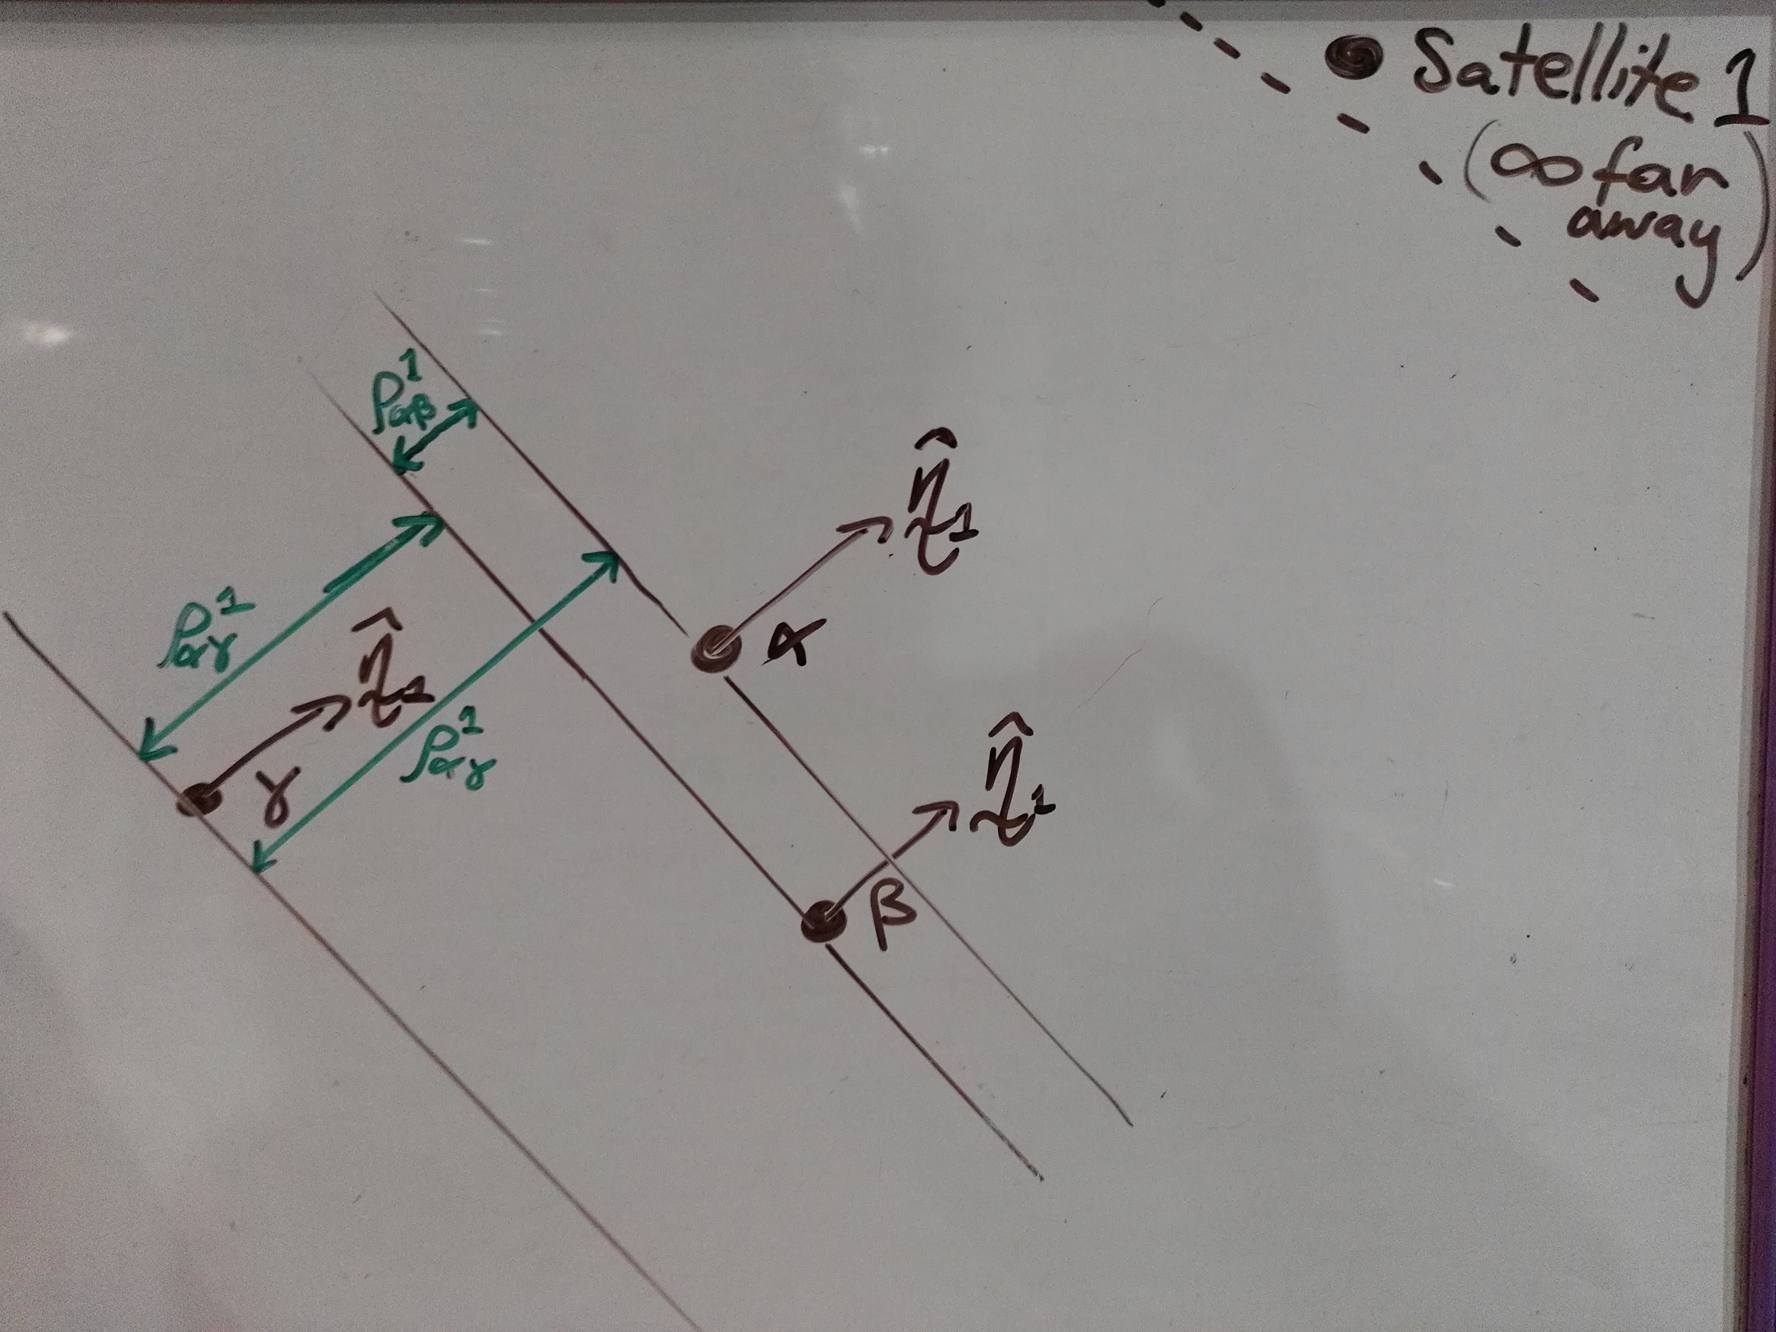
\includegraphics[width=0.7\linewidth]{ChapterLiteratureReview/overall_singleS_multiR.jpg}
\end{figure}

With multiple satellites in view, the intersection of planes for a particular receiver is the position of the receiver.
\begin{figure}[h]
\centering
\caption{}
\label{fig:overall_multiS_duelR}
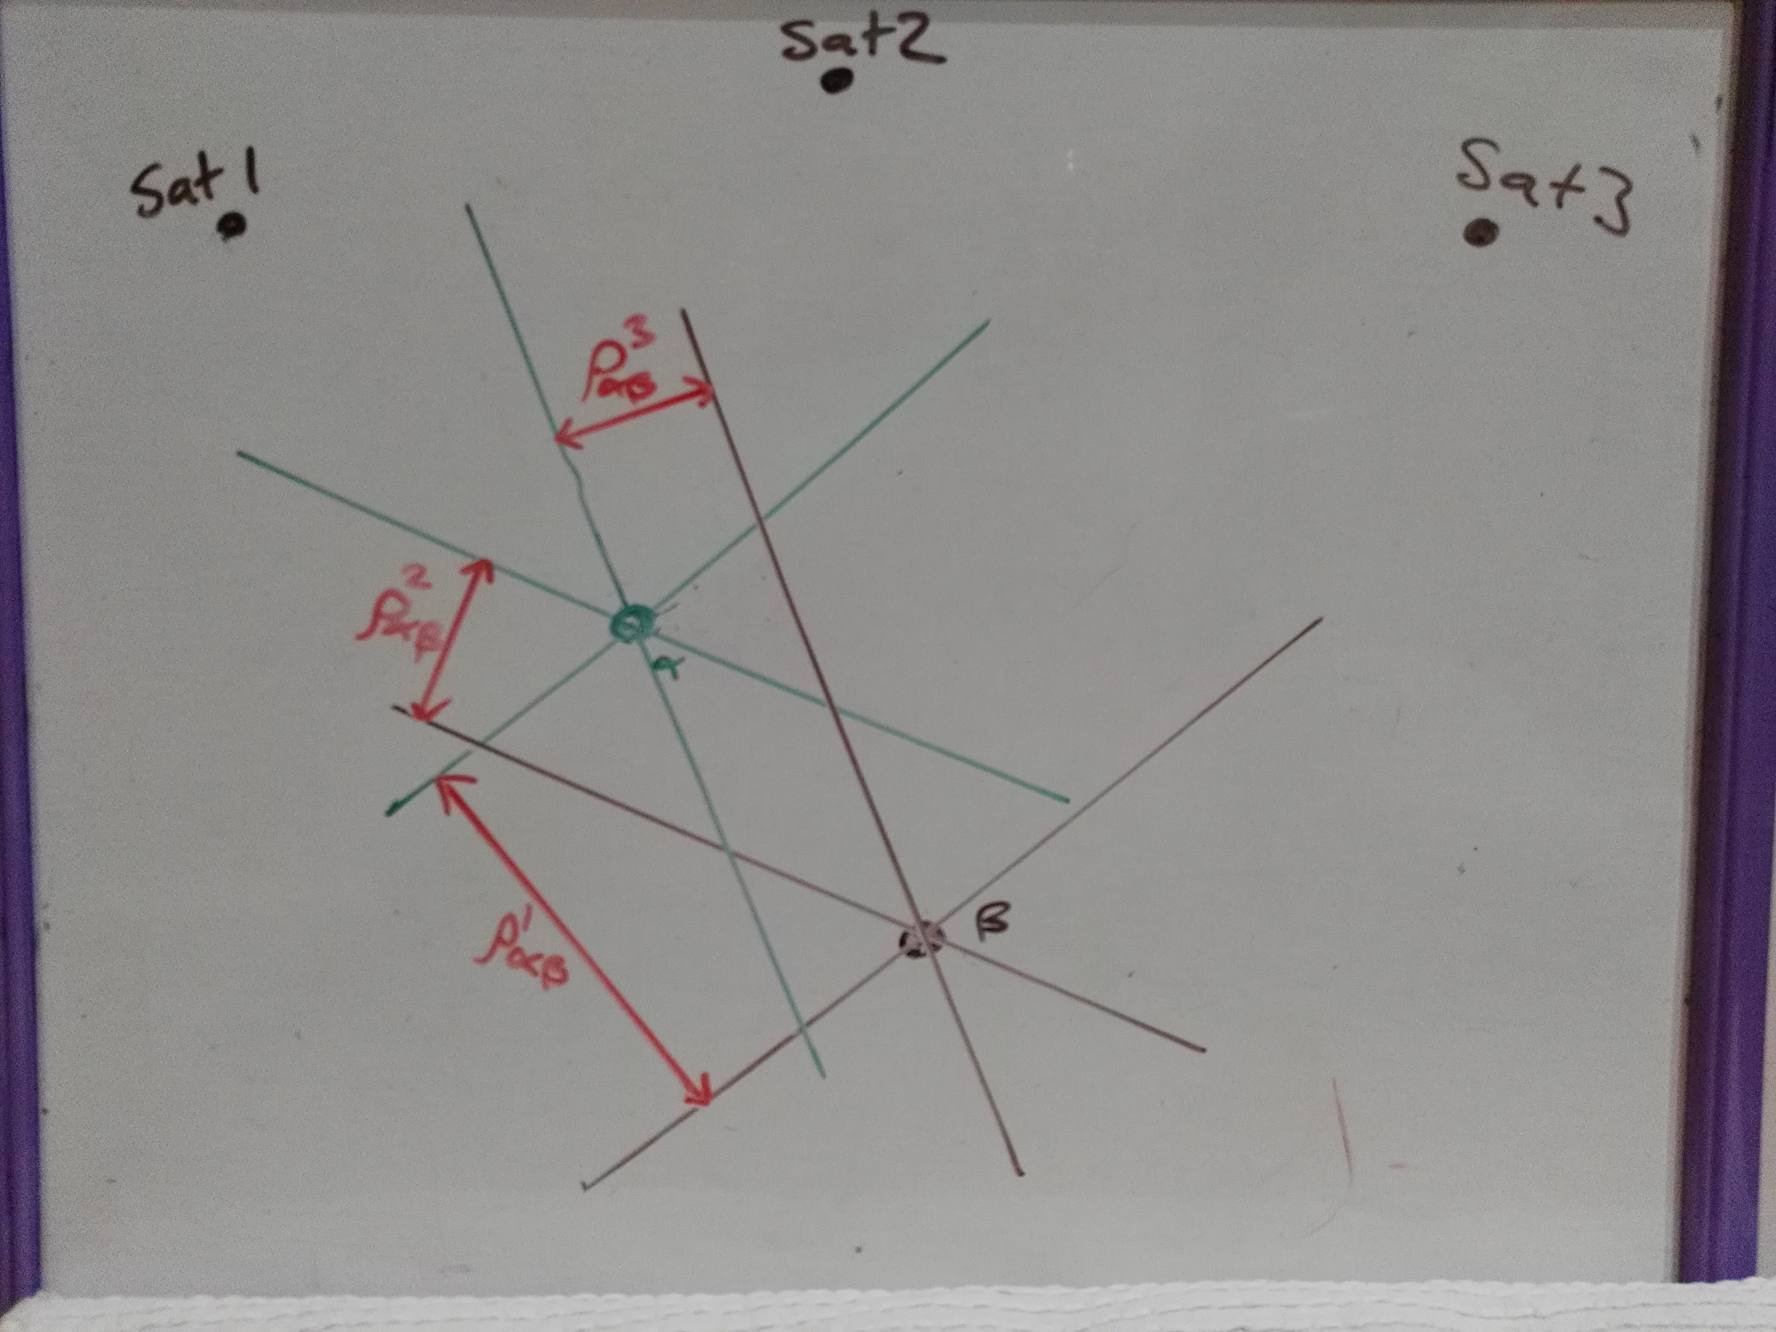
\includegraphics[width=0.7\linewidth]{ChapterLiteratureReview/overall_multiS_duelR.jpg}
\end{figure}

With this strategy, some of the errors that plague the absolute position are negated for the relative position. 
\begin{eqnarray}
\rho_i = \rho_n -cb_\omega + c(T_s + I_s+\nu_s+b_s)
\end{eqnarray}
where $\rho_n$ is the real range with the following sources of error; $b_\omega$ is the receiver clock bias, $T_s$ is the tropospheric error, $I_s$ is the ionospheric error, $\nu_s$ is the relativistic error and $b_s$ is the satellite clock bias.








% small






%??Topical organisation with inverted pyramid substructure
% \subsection{GNSS Localisation}
% Global Navigation Satellite System (GNSS) 
% - lower update rates $\approx$1Hz\\
% - accuracy/precision? not good enough for these applications\\
% - not good for indoor environments as signals are weak\\
% - used differentiated gnss to solve for integer ambiguity across multiple mobile platforms on the go \cite{GNSS_difftrack} \cite{GNSS_intamb}\\
% - multipath/atmospheric error estimation \\
% - multiple receivers across the multiplayers \cite{GNSS_multi} \\

% 	%% types of precision gnss locations 
% - double differentiating - requires same satellites
% - pvt position velocity and precise time	% Chapter 2
%!TEX root = ../Thesis.tex

\def\chapdir{./ChapterPerception}

\chapter{Algorithm Solution}\label{ch:perception}

%%%%%%%%%%%%%%%%%%%% Introduction %%%%%%%%%%%%%%%%%%%
The common theme throughout the literature is to use differencing to minimise errors, both through time and space.

For a single receiver, differencing through time 

For a single receiver differencing through space, a second known location is still required. This is set up externally and services a set area.

However for multiple receivers, spacial differencing is available. Even though with multiple receivers there is the added pre-processing with the sending of data between nodes and computation for epoch alignment. When differencing through time, the epoch alignment is required at the receiver end. That is, to manipulate the measurements as if the receivers took readings at the same time. Depending on how precise the alignment required for a system is, the computation time may require a numerical iteration solution.

When double-differencing, that is for both time and space for a single receiver.

When differencing through space between the receivers, the epoch alignment is required at the satellite end. The time the satellite sent the 
- make some ideas for when the receivers are moving - your giving the time of the positions between the receivers as different 



\section{Proposed Planar Intersection Algorithm}
- Fit better in the next chapter, put in references to literature
- these are assumptions, heres why, rationale, these ppl also did it

Following the literature, the two main options for increasing the accuracy is extensive modelling of the errors, or some type of differencing algorithm. Error modelling requires external hardware, internet connection and extra computation time which increases the budget requirements. Whereas 



This new algorithm is derived from taking the difference in pseudorange between multiple receivers from one satellite and expressing the distances as planes.
\begin{figure}[h]
\centering
\caption{2D representation}
\label{fig:overall_singleS_multiR}
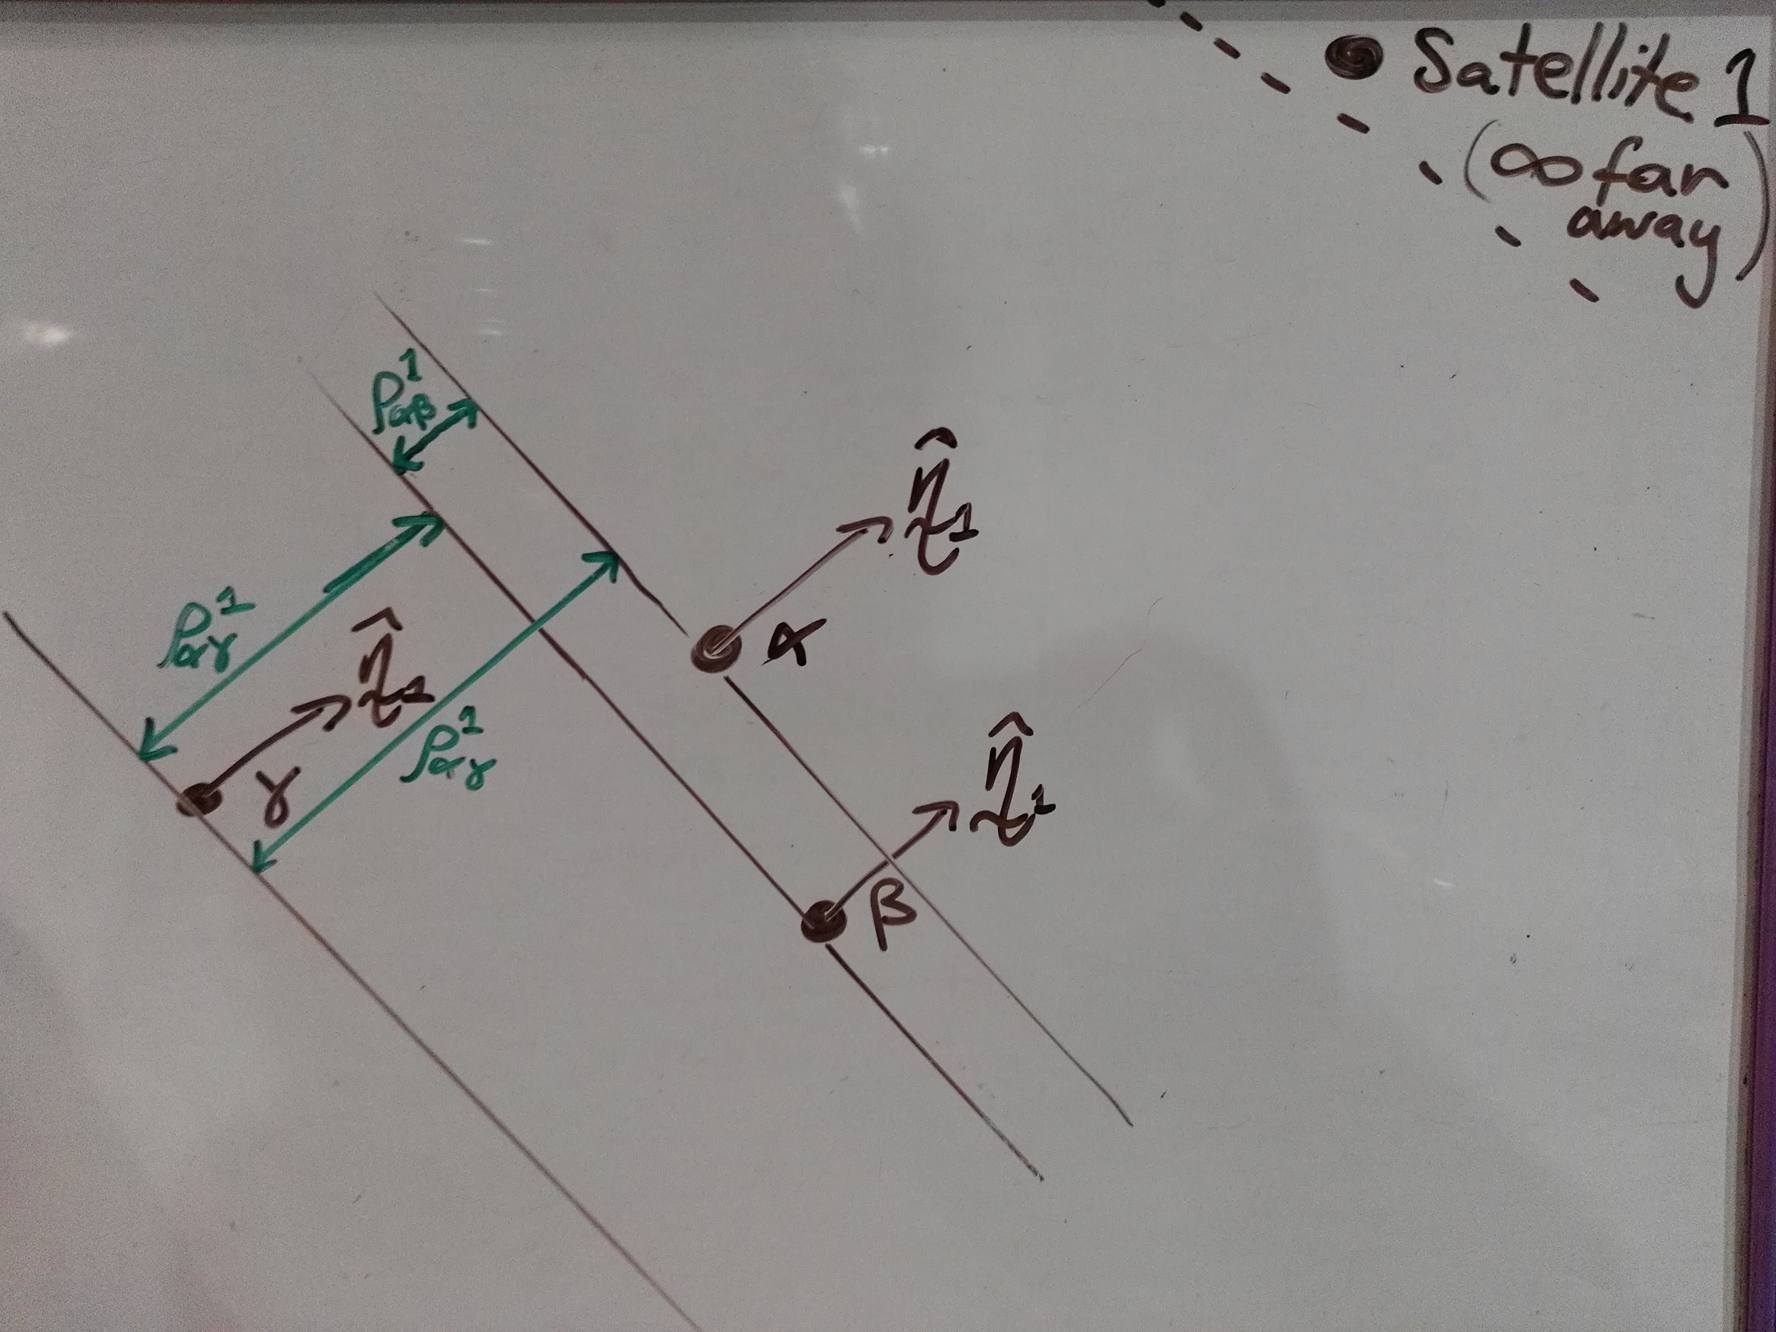
\includegraphics[width=0.7\linewidth]{ChapterLiteratureReview/overall_singleS_multiR.jpg}
\end{figure}

With multiple satellites in view, the intersection of planes for a particular receiver is the position of the receiver.
\begin{figure}[h]
\centering
\caption{}
\label{fig:overall_multiS_duelR}
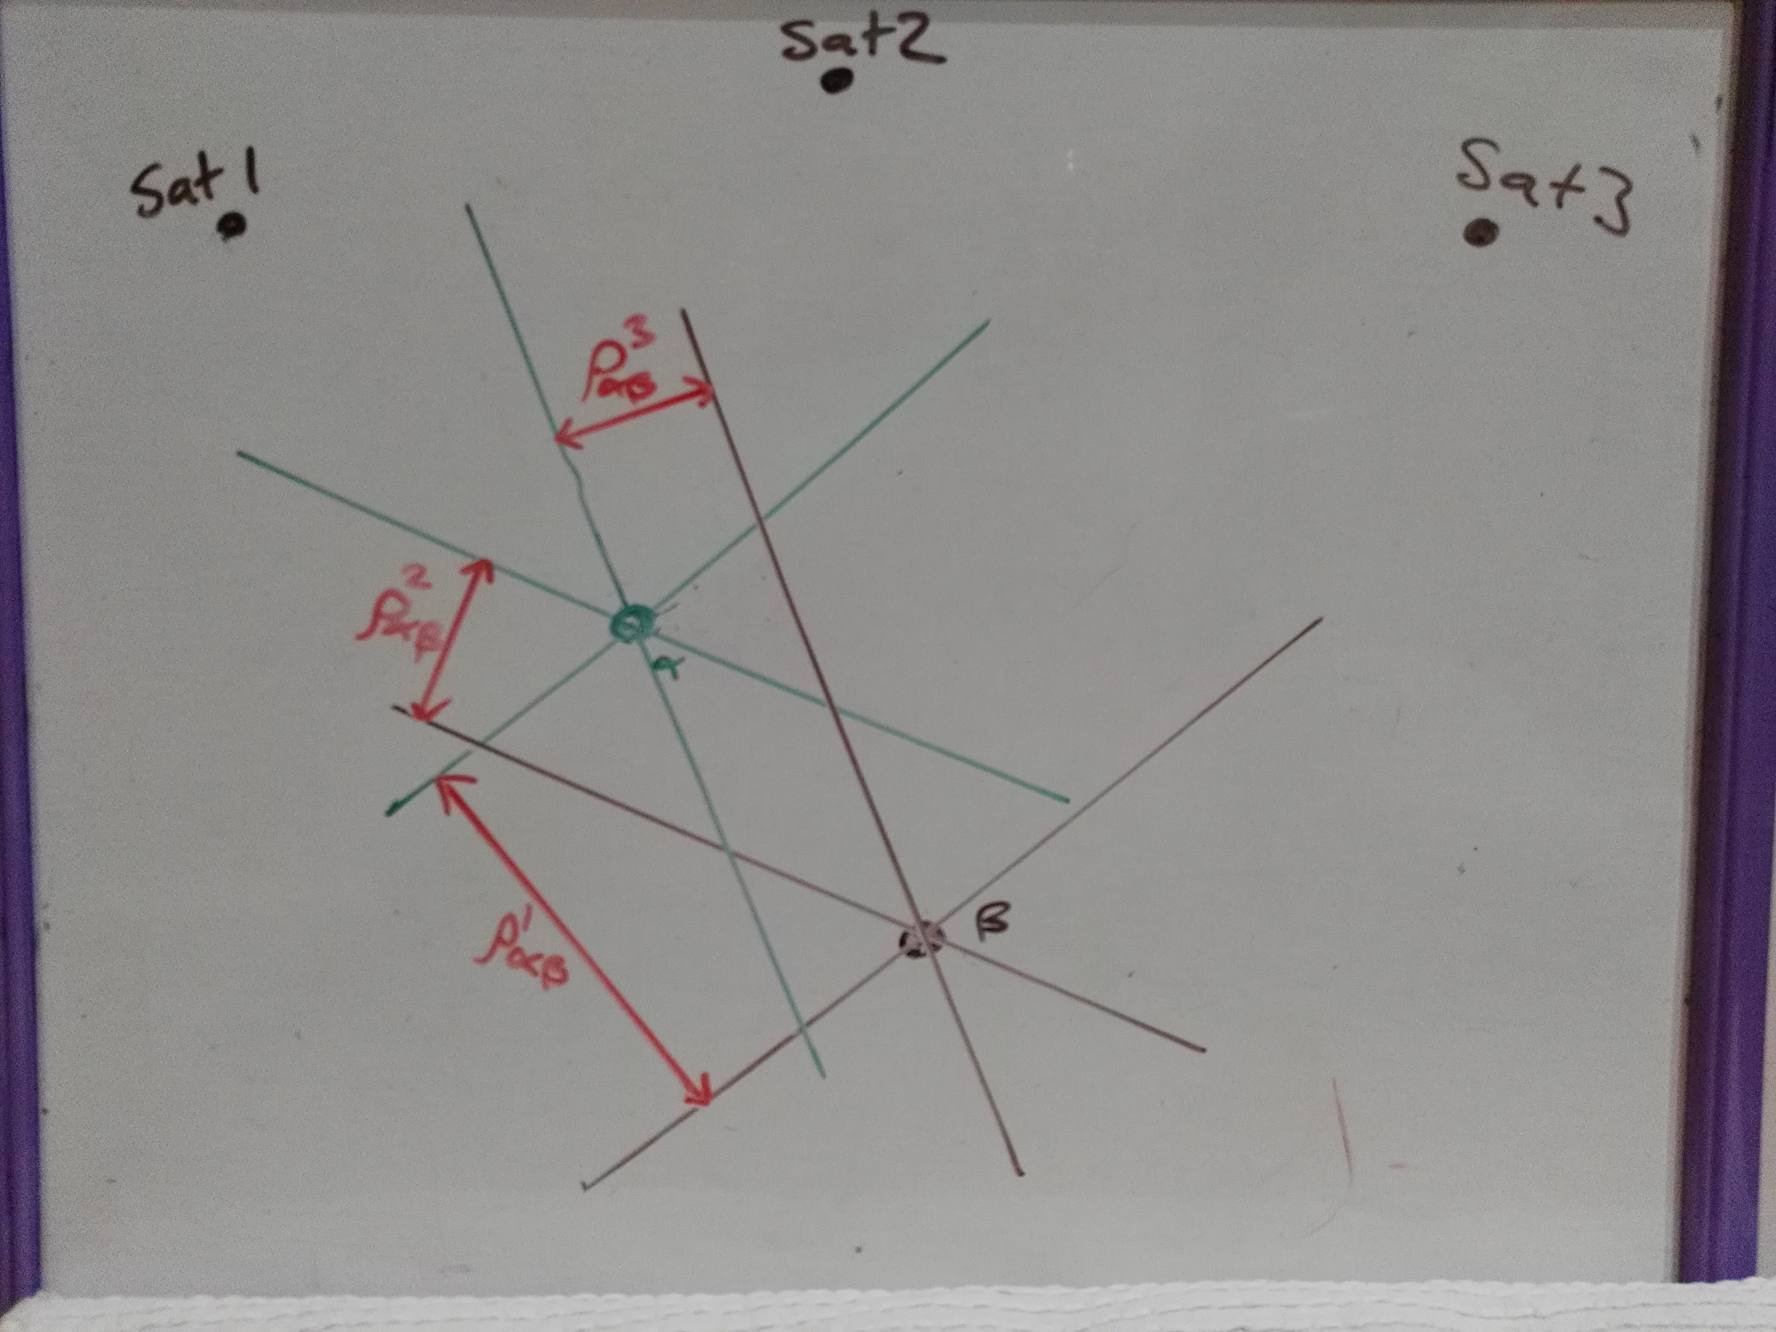
\includegraphics[width=0.7\linewidth]{ChapterLiteratureReview/overall_multiS_duelR.jpg}
\end{figure}

With this strategy, some of the errors that plague the absolute position are negated for the relative position. 
\begin{eqnarray}
\rho_i = \rho_n -cb_\omega + c(T_s + I_s+\nu_s+b_s)
\end{eqnarray}
where $\rho_n$ is the real range with the following sources of error; $b_\omega$ is the receiver clock bias, $T_s$ is the tropospheric error, $I_s$ is the ionospheric error, $\nu_s$ is the relativistic error and $b_s$ is the satellite clock bias.




%%%%%%%%%%%%%%%%%%%% Content Sections %%%%%%%%%%%%%%%%%%%

%!TEX root = ../Thesis.tex

\section{Assumptions}
All the assumptions are based on each other so need a pre-statement

\subsection{Approximate Global Location}
An approximate location is required for where the system is on the Earth within 1 km of all of the receivers. This is to calculate the normal direction vectors to each of the satellites. A simple solution to this is to set the reference receiver to calculate it's absolute position first using NLLS. This will give the system a reference of within 20 m at worst, well within the acceptable parameters.


\subsection{Static Receivers}
All receivers are assumed to be static for the time in between all receivers to get a sample reading. This makes for an easier transform to align the satellite positions to a common epoch. It also ignores the problem of how the pseudorange from each receiver would be sent to either all of the receivers or to a central device for computation and the time delay associated with that. \\

For the dynamic case, it is likely that the data would be a part of a system containing other signals that describe the motion such as dead reckoning. In that case, the location of the receiver at the common epoch time can be back calculated to minimise the dynamic error. The incorporation of moving receivers is an area to explore for future work on the algorithm. However, there are existing algorithms in the literature XX where the relative motion is tracked with sub meter accuracy that may be more appropriate for complex dynamic systems.


\subsection{Parallel plane assumption}
It as assumed for the plane equations that all receivers point to a satellite along the same vector. This is valid for a dispersion of receivers for 10km for an error of XX. This is synonymous to if the satellites were at infinity and all the receiver vectors are parallel to a satellite


\begin{eqnarray}
\delta &=& \tan^{-1}\left(\frac{d}{a}\right) \label{Eq:parplane delta}\\
e &=& 2d\tan\delta \label{Eq: parplane e(d)}\\
\eqref{Eq:parplane delta} \& \eqref{Eq: parplane e(d)}\Rightarrow e&=&\frac{2d^2}{a} \label{Eq:squarerel}
\end{eqnarray}
Where a is the altitude, d is the distance between two receivers and e is the error in the plane created. The worst configuration for error in the vector normal to the plane is if the satellite is directly above the receivers at the smallest distance from the Earth in orbit, $a>20000\;km$. For d=5 km the perpendicular error is 2.5 m





%!TEX root = ../Thesis.tex

\section{Epoch Alignment} \label{sec:epochalignment}

A single sample of pseudoranges from any two receivers will not be taken at the exact same time without a connecting network to implement control. This increases the setup requirements which in turn increases the cost of the system and reduces the ease of compatibility with different receivers. The earliest time between all the receivers will be used as the time reference point called common epoch. The satellite position in the future time steps were backcalculated to find the difference in the pseudorange. The time between receivers would be a maximum of one second, as the slowest sampling time is typically 1 Hz. This extra distance is only in the vacuum of space and is not affected by potential nonlinear affects such as ionosphere and troposphere errors that affect the speed of light.\\

The known variables from the raw GPS data is the time the sample measurement was taken $t_\omega$ and the pseudorange to each visible satellite $\rho_\omega^1$ for each receiver $\omega$.

By the distributive law, Eq\eqref{Eq: epochdist} mathematically describes the vector relationship in Figure \ref{Fig:epochsync}.
\begin{eqnarray}
\hat{\eta}\cdot s + \hat{\eta}\cdot v = |\eta|  \label{Eq: epochdist}
\end{eqnarray}
The vector $s$ is the transform of the satellite from time $t_2$ to the common epoch time $t_1$. It is extracted from the navigation message of the signals.

The vector $v$ is the measured pseudorange of a receiver from a particular visible satellite at $t_2$ with an unknown direction vector. The direction vector is unknown because the position of the receiver is what is being solved for. The vector $\eta$ describes the known direction vector from the single approximate location of the geographic region to the common epoch of a particular visible satellite. It is the magnitude of $\eta$ that describes what the pseudorange would have been if the measurement was taken at the common epoch. The difference between $|\eta|-|v|$ is the correction term $\Delta\rho$, see Eq \eqref{Eq:deltarho}.
\begin{eqnarray}
\Delta \rho &=& |\eta| - |v|\\ % check -ves
\Delta \rho&=& \hat{\eta}\cdot s + \hat{\eta}\cdot v - |v|\\
\Delta \rho&=& \hat{\eta}\cdot s + |\hat{\eta}||v|\cos(\theta) - |v| \label{Eq:deltarho}
\end{eqnarray}
As |v| is >20 000 km and s is <4 km (as the maximum time between signals is 1 seconds), $\theta\approx 0$ which means $\cos\theta\approx1$. The magnitude of a unit vector is one therefore: \eqref{Eq:deltarho} simplifies to:
\begin{eqnarray}
\Delta\rho = \hat{\eta}\cdot s 
\end{eqnarray}
Because of the asynchronous time, some of the satellite correlated errors would not correlate as well as if it was from the same point in time. This is because the path through the ionosphere and troposphere is not exactly the same. 
\begin{figure}[h]
\centering
\caption{Vector Epoch Synchronisation}
\label{Fig:epochsync}
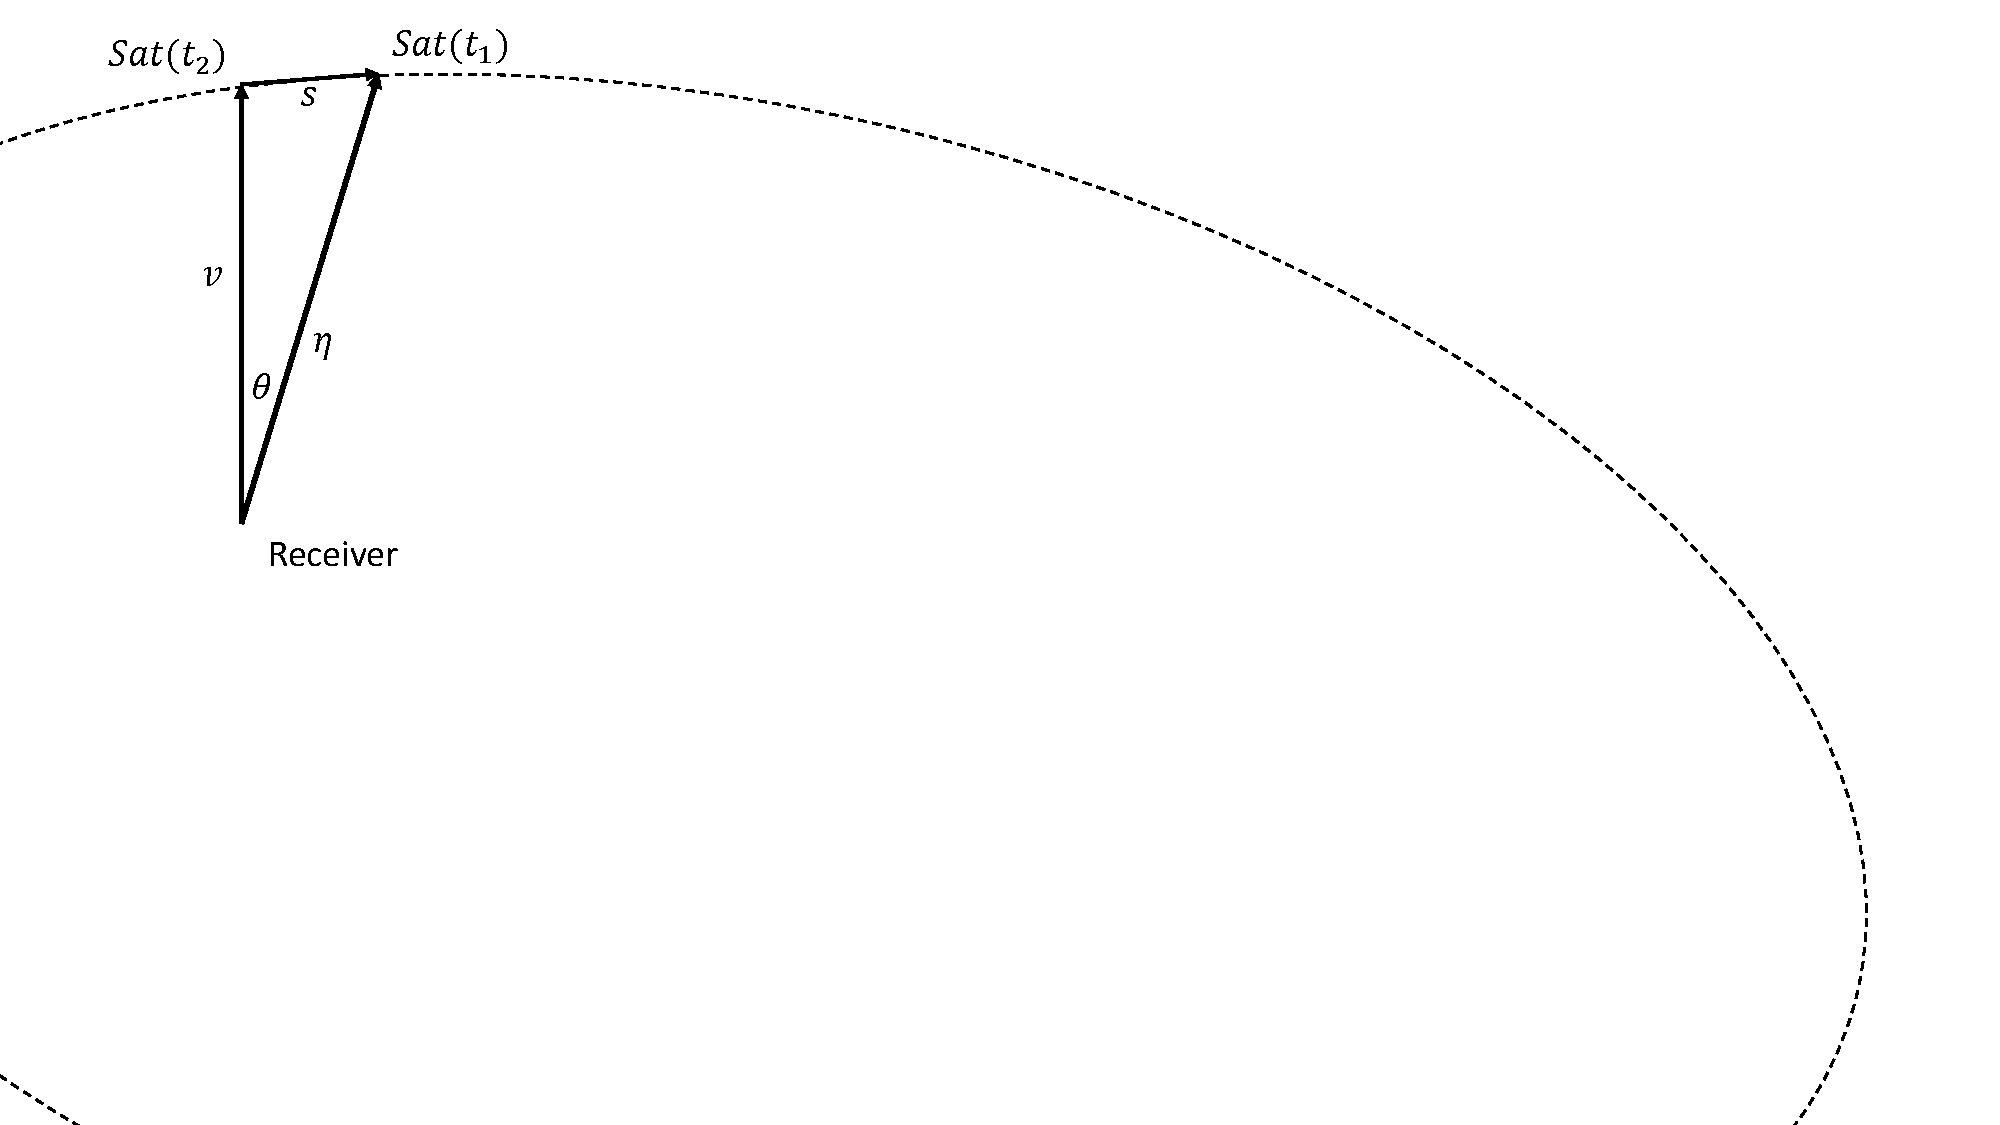
\includegraphics[trim=0 10cm 23cm 0,clip,width=0.3\linewidth]{ChapterPerception/Figures/epochalignment.pdf}
\end{figure}

% type up maths for this assumption- thats it - not an assuption, this goes into the algorithm- assumption is the asynch time described by (sample offset-time of flight) has error in position of satellite as there is error in time of flight - or do you know position of sat when sent????????









%!TEX root = ../Thesis.tex
\section{Planar Intersection Algorithm}

- assume satellite is at infinity for comparing difference in pseudorange for a particular reference satellite.\\
- use all satellites as reference satellite - no single point of failure, also not all satellites might be in view for all receivers\\
- get the normal vector between all receivers and each sat. \\
- Calculate the average normal vector.\\
- get the difference in pseudorange between all receivers along each normal vector \\
- create a plane with the normal vector with that distance\\
- solve via optimization (least squares) \\
- use clock adjustment from abs gps? or have as another optimisation variable\\
- antenna problems? misalignment?\\
- share clock bias's between solving for different reference sets? - do it one by one or all together?\\
- need to align the time of signal sent to the receivers before calculating average normal vector\\

- have weighted planes based on ? have weighted area on the planes?\\
- if one plane intercepts far away from the others then ignore it (multipath). hyperdimensional surface to minimise




% conceptual
how to send data between receivers? do it offline on a different platform?


https://www.e-education.psu.edu/geog862/node/1759 - errors in pseduorange

http://www.insidegnss.com/node/2898 - how to get pseudorange from raw data




\subsection{Algorithm}

\subsubsection{Pre-Processing}
\paragraph{Select reference receiver $\alpha$}
The receiver $\alpha$ is used as the reference location and common time in the NED frame. 
\paragraph{Collect data of one timestep from all receivers}
The raw data as well as the estimated absolute location and clock bias (what frame of reference is this?) from non-linear least squares optimisation is collected from all GNSS receivers.
\paragraph{Align to reference Epoch time}\label{timetransform}


\subsubsection{Distance Optimisation}
By optimising the distance between each pair of receivers, the error in the whole system is minimised. 
This means that the position receivers are not only relative to the reference receiver $\alpha$ but between all receivers just with the reference frame origin located at $\alpha$. It is because of this step a receiver does not need to have all the same satellites in view as all other receivers, including the designated $\alpha$.


\paragraph{Average normal Vector}
Find the average normal vector pointing to each satellite $\hat{\eta_s}$ from the receivers. The normal vector is calculated by using the position all of the satellites in view at the common time $t_{\alpha}$ as previously transformed in \ref{timetransform} and the estimated absolute position of all receivers. The average for each satellite is calculated by taking the mean across all receivers.

\paragraph{Difference in Pseudorange}
The differences in pseudorange are calculated $\Delta\rho^s_{\omega_i\omega_j}$ where s is the satellite, $\omega_i$ and $\omega_j$ are receivers $(for i<j, i\neq j)$. 

\paragraph{Optimise Pseudorange}
The pseudorange between each pair of receivers along each normal vector $\hat{\eta_s}$ creates an overdetermined linear system that is solved via least squares.
\begin{figure}
\centering
\caption{text}
\label{key}
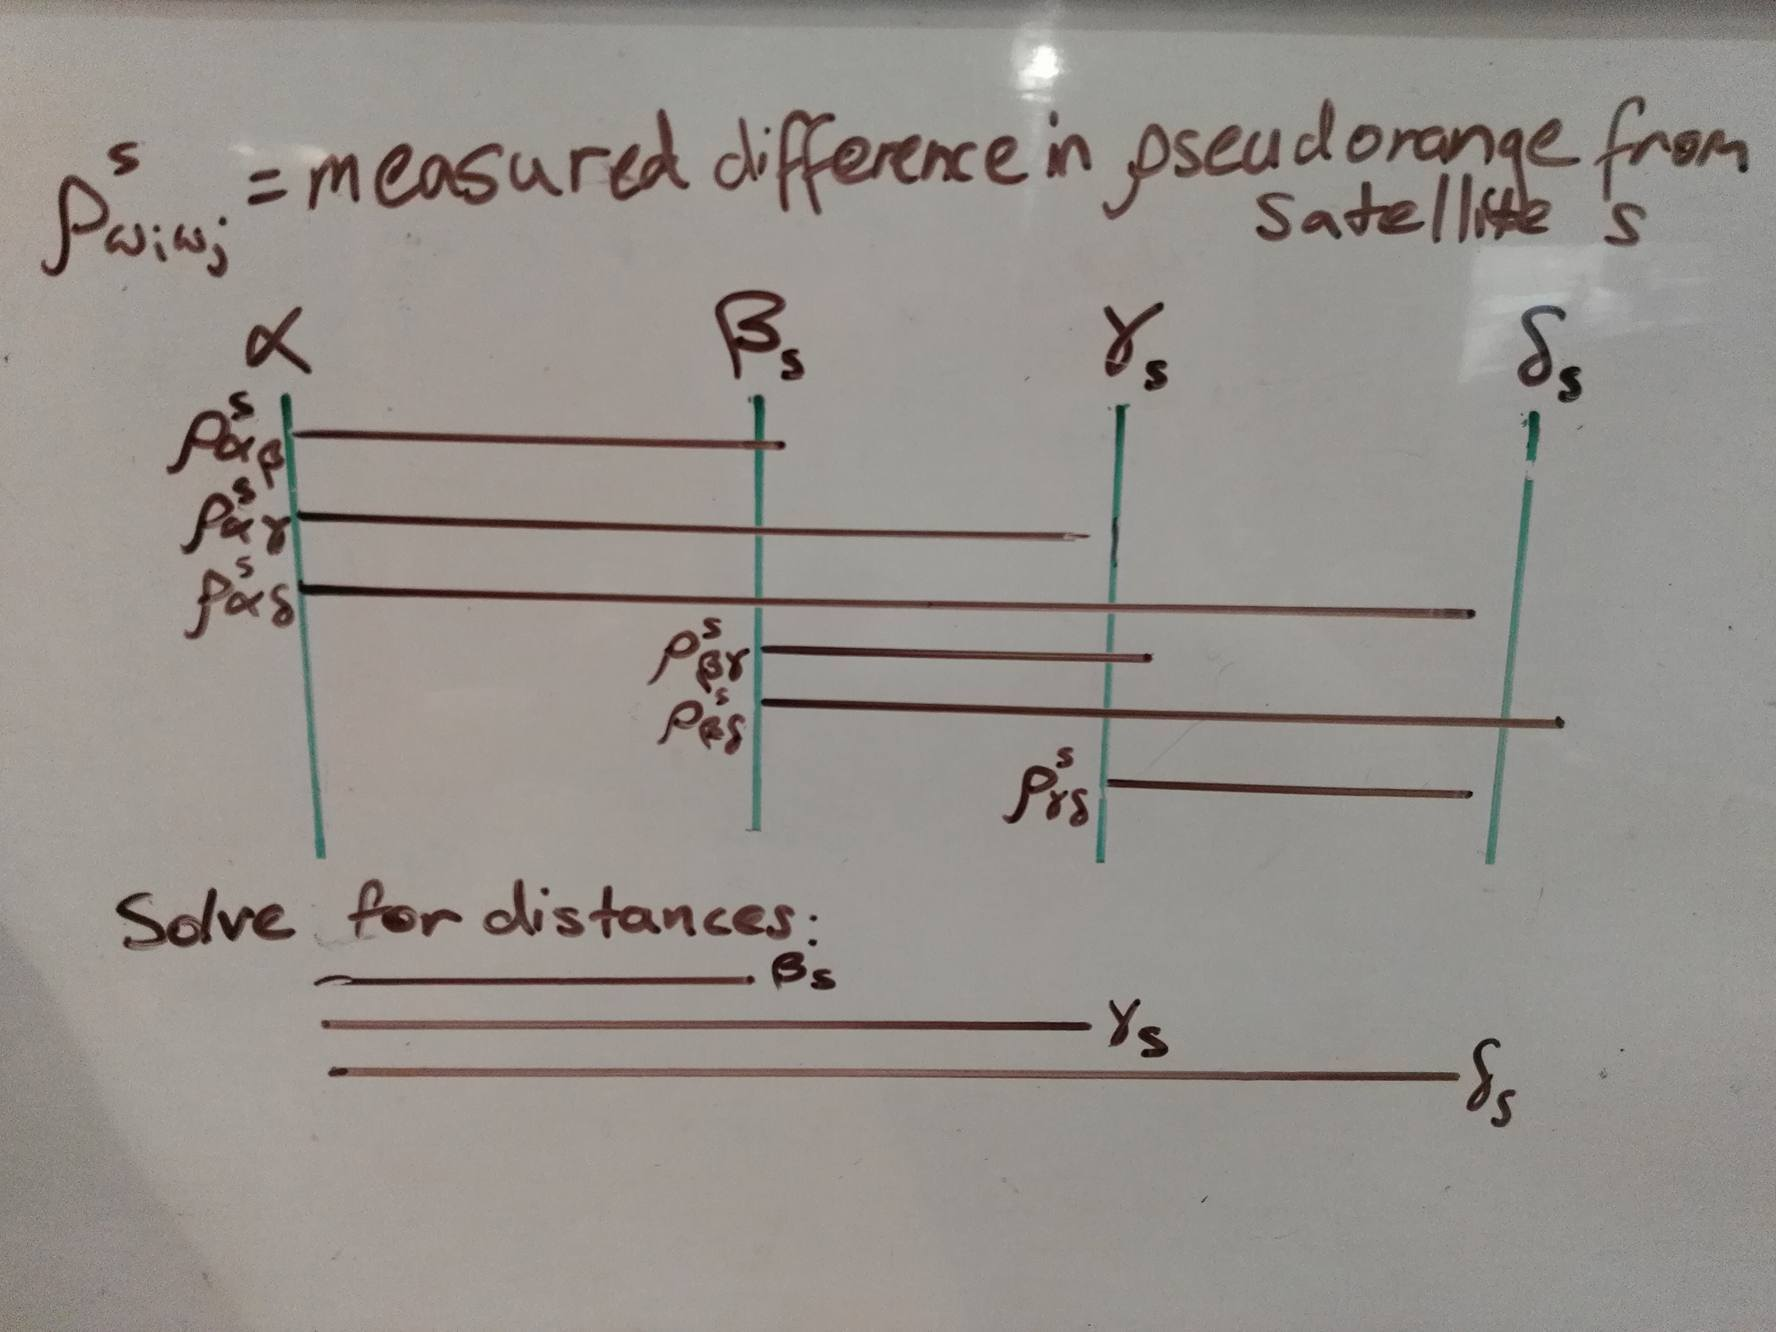
\includegraphics[width=0.7\linewidth]{ChapterPerception/Figures/solve_distances.jpg}
\end{figure}
\begin{eqnarray}
\Phi &=& \begin{bmatrix}
0 & -1 & 0 & ...\\
0 & 0 & -1 & ...\\
... & ... & ... & ... \\
1 & -1 & 0 & ...\\
1 & 0 & -1 & ...\\
\hdotsfor{4} \\
0 & 1 & -1 & ...
\end{bmatrix} \\
%
\Omega_s &=& \begin{bmatrix}
\beta_s \\
\gamma_s\\
\delta_s \\
\vdots
\end{bmatrix} \\
%
\rho_s &=& \begin{bmatrix}
\rho_{\alpha\omega_1}\\
\rho_{\alpha\omega_2}\\
\hdotsfor{1}\\
\rho_{\omega_1\omega_2}\\
\rho_{\omega_1\omega_3}\\
\vdots
\end{bmatrix} 
\end{eqnarray}

\begin{eqnarray}
\Phi\times\Omega_s = \rho_s
\end{eqnarray}
Solve by linear least squares for an overdetermined system by the pseudo inverse matrix
\begin{eqnarray}
\Omega_s = (\Phi^T\Phi)^{-1}\Phi^T\rho_s
\end{eqnarray}

\subsubsection{Point Optimisation}
\paragraph{Create Planes}
Create sets of planes for each receiver $\omega$ from the normal vectors $\hat{\eta_s}$ and the set of distances from the reference point $\alpha$ to receiver $\omega$ along each of the normal vectors denoted $\Omega_\omega$.

The equation of a plane is $Ax+By+Cz+D=0$ where the coefficients [A,B,C] describe the normal vector of the plane and the coefficient D sets the plane in 3D space along the vector. As the normal vector is already calculated for each satellite, only the D coefficient must be solved for each receiver and satellite pair. 
\begin{eqnarray}
P_\omega^s &=& (i\cdot\hat{\eta_s})x + (j\cdot\hat{\eta_s})y + (k\cdot\hat{\eta_s})z + D_\omega^s \label{genplane}\\
P_\omega^s &=& I\cdot H +D_\omega\\
\end{eqnarray}
Where $I = x\hat{\textbf{i}}+y\hat{\textbf{j}}+z\hat{\textbf{k}}$ is the *identity* vector and H is a matrix of normal vectors to each satellite:
\begin{eqnarray}
H = \begin{bmatrix}
\hat{\eta_1} \\
\hat{\eta_2} \\
\vdots\\
\hat{\eta_n}
\end{bmatrix}
\end{eqnarray}
The coefficient D can be calculated by finding a point on the plane $f_\omega^s$, then substituting it into \eqref{genplane} for x,y,z. The point of the plane is calculated by moving along the normal vector by the optimised pseudo distance from the reference point \eqref{Eq:f}.
\begin{eqnarray}
f_\omega^s &=& \Delta_\omega^s\hat{\eta_s} \label{Eq:f}\\
P_\omega^s &=& \hat{\eta_s}\cdot f_\omega^s +D_\omega^s = 0\\
D_\omega^s &=& -\hat{\eta_s}\cdot f_\omega^s\\
D_\omega^s &=& -\Delta_\omega^s ||\hat{\eta_s}|| \\
||\hat{\eta_s}|| &=& 1\\
D_\omega^s &=& -\Delta_\omega^s\\
\Rightarrow P_\omega^s &=& I\cdot H -\Omega_\omega
\end{eqnarray}

\begin{figure}[h]
\centering
\caption{Find position $f_\omega^s$ on the plane}
\label{fig:pointonplane}
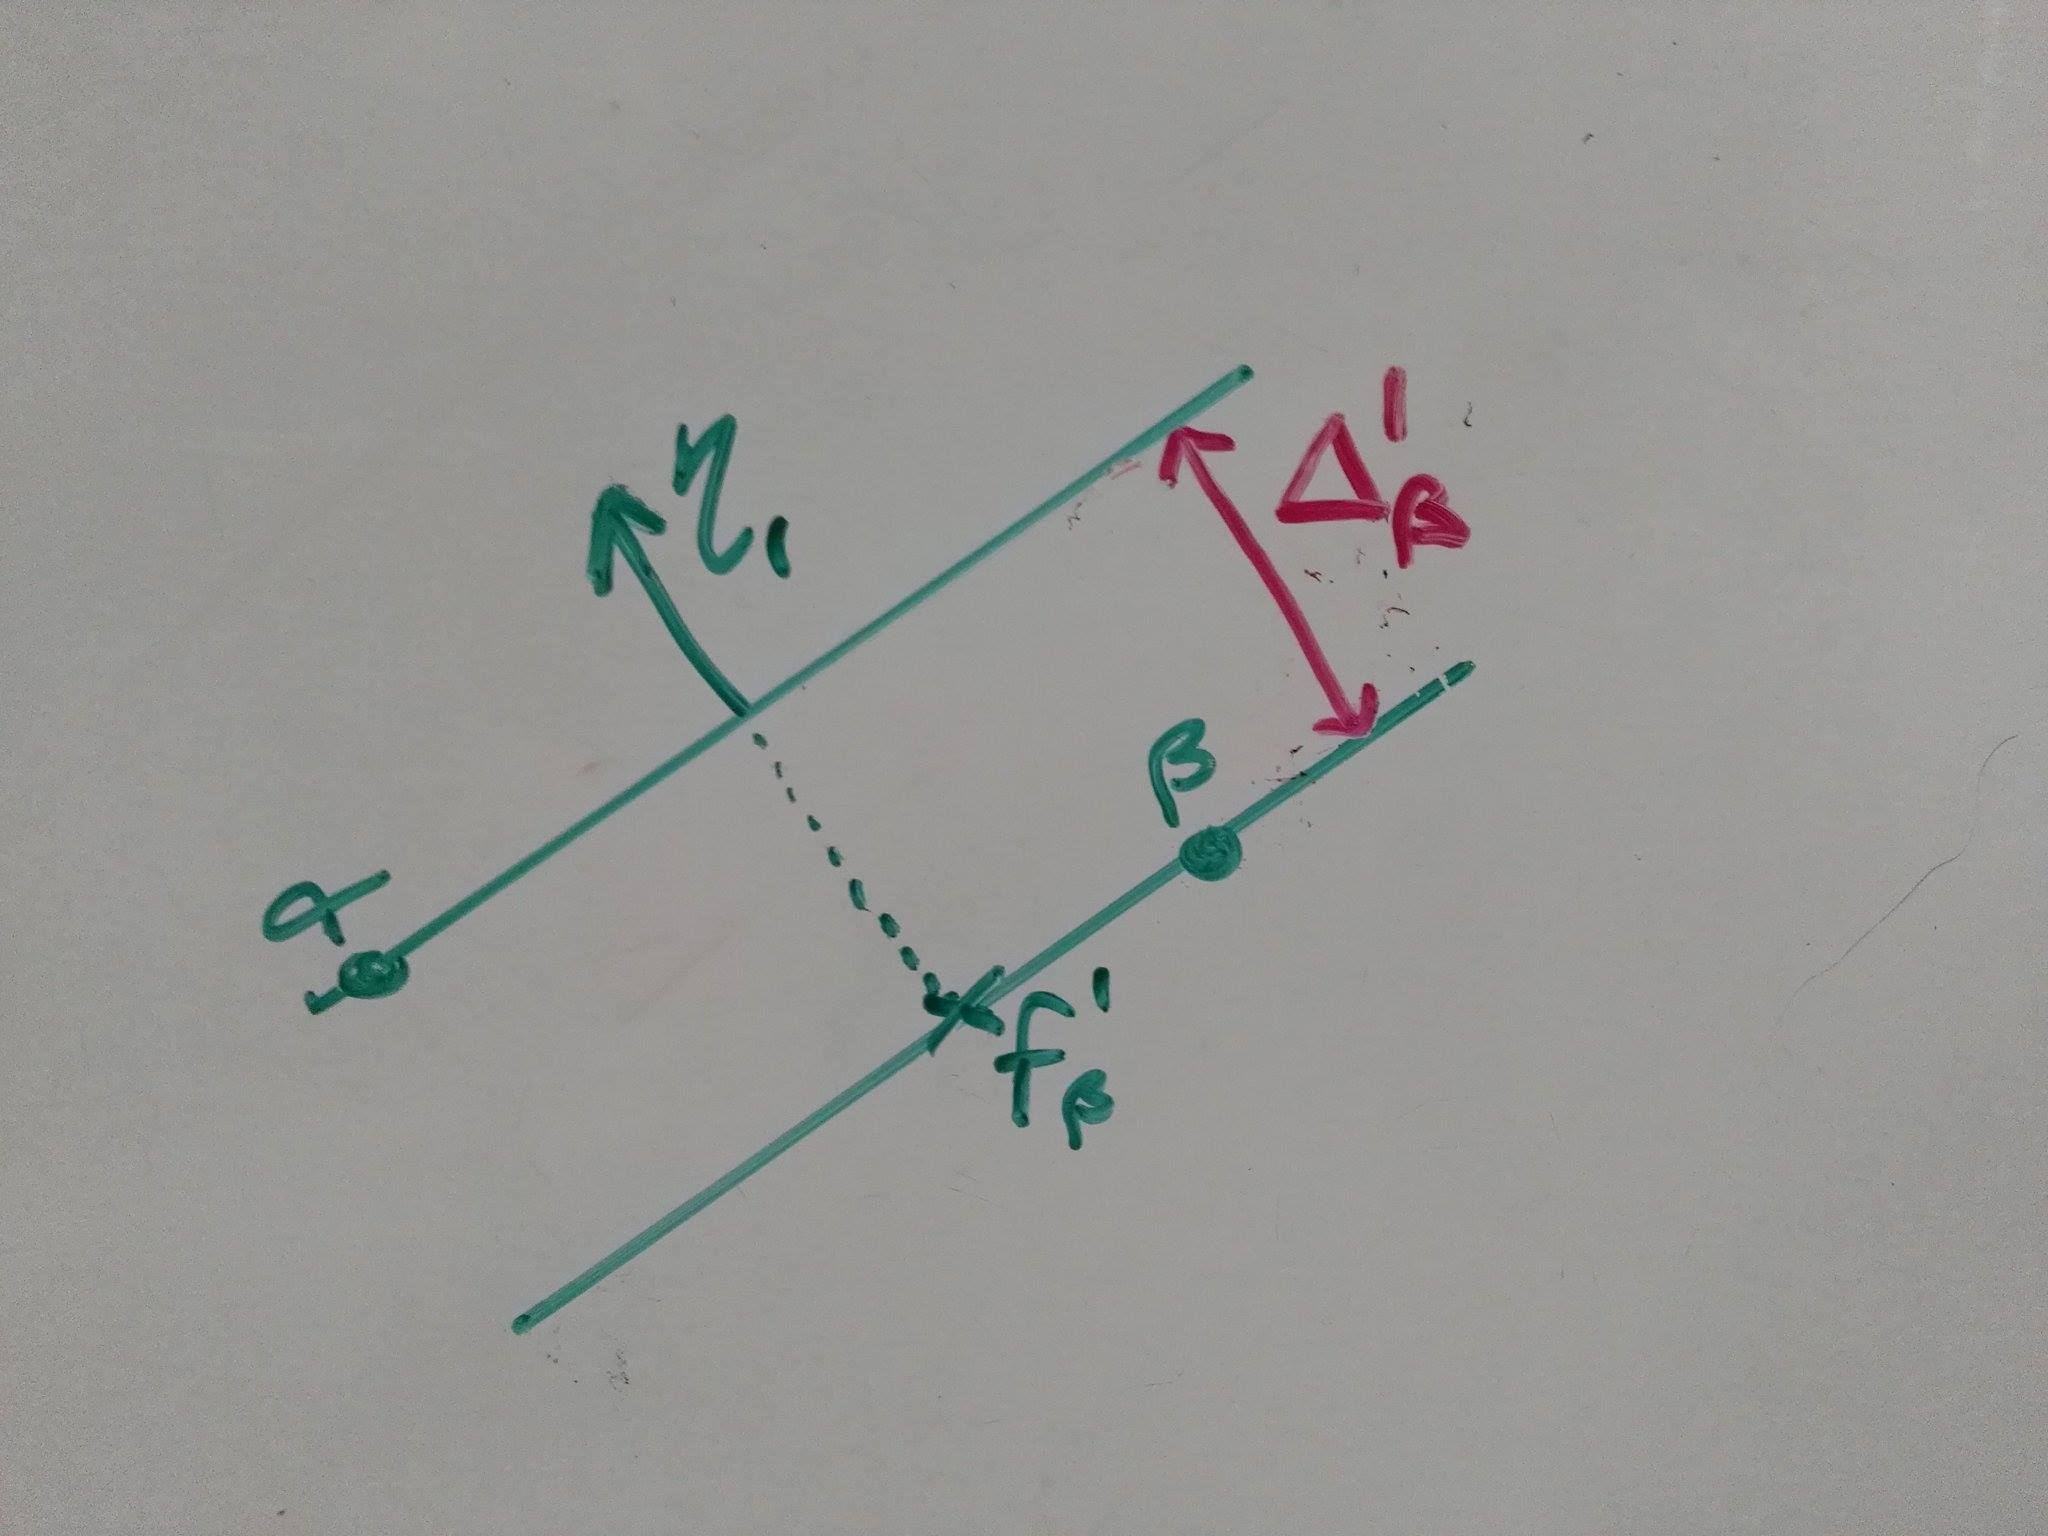
\includegraphics[width=0.7\linewidth]{ChapterPerception/Figures/pointonplane}
\end{figure}






$\Omega_\omega$ is a vector of optimised pseudo-distances from reference $\alpha$ to receiver $\omega$ for all satellites $s\in{1,2...n}$
\begin{eqnarray}
\Omega_\omega = \begin{bmatrix}
\Delta_{\omega}^1 \\
\Delta_{\omega}^2 \\
\vdots\\
\Delta_{\omega}^n \\
\end{bmatrix}
\end{eqnarray}
Where $\Omega_s$ is the vector of optimised pseudo-distances from $\alpha$ to each receiver $\omega\in1,2...m$ for a single satellite s:
\begin{eqnarray}
\Omega_s = \begin{bmatrix}
\Delta_{\omega_1}^s \\
\Delta_{\omega_2}^s \\
\vdots\\
\Delta_{\omega_m}^s \\
\end{bmatrix}
\end{eqnarray}


\paragraph{Solve for Intersection}
As the system of homogeneous linear equations is overdetermined, it can be solved using singular value decomposition to find a point that has the minimum residuals from all of the planes in its set $P_\omega$. Each set of planes for a particular receiver is independent to all other receivers. The vector $X_\omega$ describes the position of receiver $\omega$ in NED coordinates and $\tau_\omega$ describes a final receiver clock bias that alters the displacement of all the planes in the set $P_\omega$ by the same parameter.
\begin{eqnarray}
X_\omega &=& \begin{bmatrix}
x_\omega \\y_\omega \\ z_\omega \\ \tau_\omega
\end{bmatrix}\\
P_\omega X_\omega &=& D_\omega \\
\end{eqnarray}
In order to solve all of the receivers with the least amount of error in the whole system, all of the position vectors $X_\omega$ are solved at the same time. The reference planes of $\alpha$ must be included as a constraint on the system. All of the clock biases are also constrained with the clock bias from $\tau_\alpha$, see \eqref{Eq: P with alphat}.
The receiver clock bias only affects the equation of the planes by altering the constant as a change in the pseudorange has no affect over the angle of the plane. Each receiver clock bias alters all the planes associated with that receiver proportionally. 
\begin{eqnarray}
P_\omega^s &=& (i\cdot\hat{\eta_s})x + (j\cdot\hat{\eta_s})y + (k\cdot\hat{\eta_s})z + D_\omega^s + (\tau_\omega-\tau_\alpha) \label{Eq: P with alphat}\\
\end{eqnarray}
 



%%%%%%%%%%%%%%%%%%%% Conclusions %%%%%%%%%%%%%%%%%%%

\section{Summary}

\Autoref{ch:estimation} and \autoref{ch:experiments} take things to a more advanced level.
				% Chapter 3
%!TEX root = ../Thesis.tex

\def\chapdir{./ChapterExperiments}

\chapter{Simulation and Analysis}\label{ch:experiments}

%%%%%%%%%%%%%%%%%%%% Introduction %%%%%%%%%%%%%%%%%%%
A simulation was built in matlab to verify the assumptions and analyse the performance and limitations of the algorithm.


%%%%%%%%%%%%%%%%%%%% Content Sections %%%%%%%%%%%%%%%%%%%
%!TEX root = ../Thesis.tex

\section{Simulation Creation}\label{sec:Method}

\subsection{Creating a Simulation}
Matlab was chosen as the platform to simulate and evaluate the program due to the ease of matrix manipulation and graphical interaction.
\subsubsection{Simulate Satellite Locations}
Using real ephemeris data for the GPS constellation, the location of all of the satellites were calculated, see Table \ref{Table: eph gps data}. The approximate reference location of the network of receivers was inputed into the program as longitude, latitude, height geocentric coordinate system. The satellite positions were transformed to the local tangent plane of the reference location in polar coordinates. The satellites that had an elevation of above 12$\deg$ were selected as potential visible satellites. This lower elevation limit was selected to minimised multipath effects that would likely occur at ground level \textcolor{red}{REF}. 
\begin{table}
\centering
\caption{Ephemeris data for GPS constellation}
\label{Table: eph gps data}
\begin{tabular}{|c|c|}
\hline
Orbital parameters & Value \\\hline
\end{tabular}
\end{table}





\subsubsection{True Location of Receivers}
The dispersion of receivers from $\alpha$ is a variable to the program. The actual displacement is calculated by multiplying the dispersion magnitude by a uniformly distributed random vector ranging from [0,1] in three dimensions for all remaining receivers in North-East-Down (NED) frame localised at $\alpha$. The positions were then transformed to the global ECEF frame.

\subsubsection{Calculation of Pseudorange}
In ECEF frame, the instantaneous distance between each visible satellite and each receiver was calculated. The errors were simulated by adding random distance proportional to error models in the literature to each individual satellite, see Table \ref{Table:mag errors}. The errors followed the structure in Eq\eqref{Eq: errorstruc}

For the error analysis, the errors associated with the pseudorange were divided into three sections; satellite correlated errors, receiver correlated errors and random errors. For the satellite correlated errors, the same amount was added to the true range for each receiver from a single satellite. For the receiver correlated errors, the same amount was added to the true range for each satellite from a single receiver.  
All errors were an addition to the pseudorange, so that how each type of error affected the algorithms 
%In the literature, the errors were expressed in meters which were converted to seconds.
\begin{eqnarray}
Error(seconds) = magnitude + 10\times magnitude\times rand(elements) \label{Eq: errorstruc}
\end{eqnarray}
Where \textit{rand} is an inbuilt matlab function that returns a value on the domain [0,1] in a standard uniform distribution.

\begin{table}
\centering
\caption{Magnitude of simulated errors}
\label{Table:mag errors}
\begin{tabular}{|c|c|}
\hline
Error Source & meters \\\hline
\end{tabular}
\end{table}



\subsubsection{Planar Algorithm}
The normal vector was


- what data is it using from receiver? psudorange, time\\

- what errors to include and how to incorporate into the simulation.\\
- how to include the different(asynchronous ) time received for all receivers-> is for the one receiver \\
- how extra receivers affects computational time/ accuracy\\
- how number of sats affect comp time/accuracy\\
- configuration of sats\\
- large multipath affects\\
- no receiver sees the same sat? - does it just output the relative difference between abs values? -> incorrect? just have it fail? not actually implementing, can control the environment\\
- distance of receivers apart\\
- configuration of receivers


- what data received and how to simulate misaligned timing between receivers\\
- what magnitude are the errors and how to simulate them\\
- simulate the errors individually (to see how each type affects the sim - convergence time and accuracy) and/or all errors at once


\subsection{Evaluation} % how to evaluate
The expected error due to the assumptions were outlined in Section XX. To evaluate the parallel plane assumption, two receivers were a set distance apart.


\paragraph{Dilution of Precision}
The dilution of precision (DOP) is a measure of how the geometry of the satellites affect the position measurement precision. It is used in GNSS to evaluate how much error there may be in a measurement. Figure \ref{Fig: GDOP abstract} shows two different configurations of satellites in the 2D circular solution case. With some error bounds as shown in B and C, the solution can lie anywhere in the green area. Due to the geometry configuration of the satellites in C, the area is considerably larger even though the error bounds on the signals are the same.

\begin{figure}
\centering
\caption{Geometric Dilution of Precision}
\label{Fig: GDOP abstract}
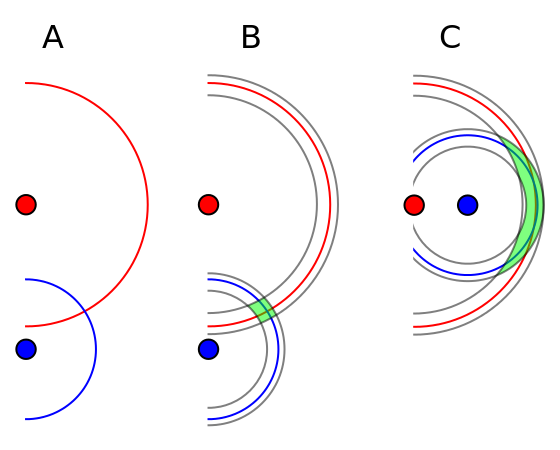
\includegraphics[width=0.7\linewidth]{ChapterExperiments/Figures/GDOP.png}
\end{figure}




- fake gps data\\
- how to simulate noise - what level SNR\\
- to calculate your own GPS location using the normal algorithm? - space 3 \\
- use real GPS locations? (and through time) -space 3\\





%!TEX root = ../Thesis.tex

\section{Method}\label{sec:Method}

\subsection{Creating a Simulation}
Matlab was chosen as the platform to simulate and evaluate the program due to the ease of matrix manipulation and graphical interaction.
\subsubsection{Simulate Satellite Locations}
Using real ephemeris data for the GPS constellation, the location of all of the satellites were calculated, see Table \ref{Table: eph gps data}. The approximate reference location of the network of receivers was inputed into the program as longitude, latitude, height geocentric coordinate system. The satellite positions were transformed to the local tangent plane of the reference location in polar coordinates. The satellites that had an elevation of above 12$\deg$ were selected as potential visible satellites. This lower elevation limit was selected to minimised multipath effects that would likely occur at ground level \textcolor{red}{REF}. 
\begin{table}
\centering
\caption{Ephemeris data for GPS constellation}
\label{Table: eph gps data}
\begin{tabular}{|c|c|}
\hline
Orbital parameters & Value \\\hline
\end{tabular}
\end{table}

\subsubsection{True Location of Receivers}
The dispersion of receivers from $\alpha$ is a variable to the program. The actual displacement is calculated by multiplying the dispersion magnitude by a uniformly distributed random vector ranging from [0,1] in three dimensions for all remaining receivers in ECEF frame localised at $\alpha$. The positions were then transformed to the global ECEF frame.

\subsubsection{Calculation of Pseudorange}
In ECEF frame, the instantaneous distance between each visible satellite and each receiver was calculated. The errors were simulated by adding random distance proportional to error models in the literature to each individual satellite, see Table \ref{Table:mag errors}. The errors followed the structure in Eq
In the literature, the errors were expressed in meters which were converted to seconds.
\begin{eqnarray}
Error(seconds) = (Error)
\end{eqnarray}
\begin{table}
\centering
\caption{Magnitude of simulated errors}
\label{Table:mag errors}
\begin{tabular}{|c|c|}
\hline
Error Source & meters \\\hline
\end{tabular}
\end{table}

\subsubsection{Planar Algorithm}
The normal vector was


- what data is it using from receiver? psudorange, time\\

- what errors to include and how to incorporate into the simulation.\\
- how to include the different(asynchronous ) time received for all receivers-> is for the one receiver \\
- how extra receivers affects computational time/ accuracy\\
- how number of sats affect comp time/accuracy\\
- configuration of sats\\
- large multipath affects\\
- no receiver sees the same sat? - does it just output the relative difference between abs values? -> incorrect? just have it fail? not actually implementing, can control the environment\\
- distance of receivers apart\\
- configuration of receivers


- what data received and how to simulate misaligned timing between receivers\\
- what magnitude are the errors and how to simulate them\\
- simulate the errors individually (to see how each type affects the sim - convergence time and accuracy) and/or all errors at once


\subsection{Evaluation} % how to evaluate
The expected error due to the assumptions were outlined in Section XX. To evaluate the parallel plane assumption, two receivers were a set distance apart.


\paragraph{Dilution of Precision}
The dilution of precision (DOP) is a measure of how the geometry of the satellites affect the position measurement precision. It is used in GNSS to evaluate how much error there may be in a measurement. Figure \ref{Fig: GDOP abstract} shows two different configurations of satellites in the 2D circular solution case. With some error bounds as shown in B and C, the solution can lie anywhere in the green area. Due to the geometry configuration of the satellites in C, the area is considerably larger even though the error bounds on the signals are the same.

\begin{figure}
\centering
\caption{Geometric Dilution of Precision}
\label{Fig: GDOP abstract}
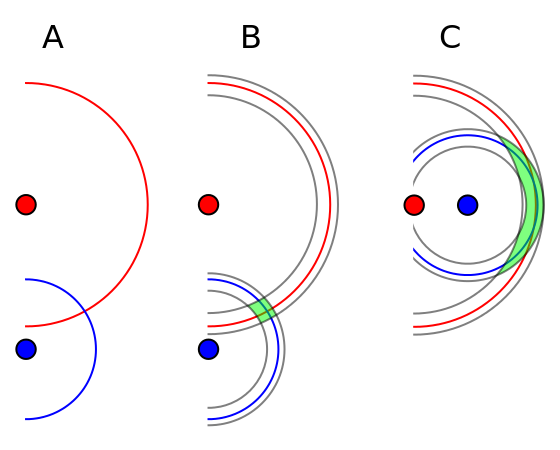
\includegraphics[width=0.7\linewidth]{ChapterExperiments/Figures/GDOP.png}
\end{figure}




- fake gps data\\
- how to simulate noise - what level SNR\\
- to calculate your own GPS location using the normal algorithm? - space 3 \\
- use real GPS locations? (and through time) -space 3\\
- vary number of satellites in view\\
- vary GDOP (good GDOP and bad)\\
- when receivers don't see the exact same satellites \\
- vary number of receivers \\
- simulate a multipath error and how does it account for it or how much error does it introduce\\

How to evaluate?:
- accuracy in relative space\\
- compare to just taking differences in absolute position \\
- between individual receivers and the total error in the whole system\\
- markov? error analysis -> cannot do precision without statistical analysis but isolate errors in x,y,z. how much worse is z than horizontal?\\
- computational time-> how does more receivers/satellites affect the comp time -> what time and space complexity?



%!TEX root = ../Thesis.tex

\section{Planar Assumption Analysis}
\subsection{Setup}
These results had no error induced in the measurements in order to analyse the effectiveness and robustness of the algorithm. No epoch alignment and no correlated or uncorrelated errors. Only two receivers were used with the reference receiver exactly at the approximate location. The second receiver was set at varied configurations of a set distance north, east and down of the reference receiver. The set distance between the receivers was varied from 1 mm to 100 km. As there are no randomly induced errors, there is no statistical analysis. The algorithm was also adjusted to not solve for a clock bias variable to see how the least squares solution adjusted the distance between planes without error in the system.\\

The satellites were configured in a small cluster to analyse how the position of the satellites relative to the configuration of the receivers affected the plane assumption. The total error and the individual component error were calculated to identify what component produces the most error for the configuration.\\

This analysis was not required to be compared to NLLS as there was no error and it would solve the system perfectly to mathematical precision.

\subsection{Discussion}
See Figure \ref{fig:plane_ALLE_north_9060}, two receiver configuration with one receiver at the approximate location and one receiver at varying distance along the north direction. The cluster of satellites were set perpendicular to the receiver configuration as it was predicted to be a configuration with less error. This isolated the error due to the plane assumption. The algorithm was compared to solving the same plane intersections but without the clock bias variable. In Figure \ref{fig:plane_ALLE_north_9060}, for distances < 1 meter, the planar algorithm solution has a consistent error two orders of magnitude larger than the solution without the clock bias. This indicates that without errors, the least squares matrix adjusts the distance between planes proportionally but will introduce errors. These errors however are on the order of micrometers ($10^{-6}$) and will be below the noise floor with any error in the system.\\

The results show that the least squares setup by constraining to the reference receiver is successful as the error is not proportional to distance below 10 m. Above 10 m the error increases for both the solutions with and without the clock bias, indicating that the error is due to the planar assumption. The slope has a gradient of $m = \log(10^4)/\log(10^2) = 2$ which means the error is proportional to the square of the distance. This was to be expected as in reality, the distance from the satellites are spheres, as stated in Eq\eqref{Eq:squarerel}. However the magnitude of error was 1 m at 10 km distance, which for localised systems is acceptable.\\

The individual component error shows where the error has come from. In Figure \ref{fig:plane_ALLE_north_9060}, it the error in the north component is much smaller than the error due to the east or down component. This is based on the satellite configuration relative to the receiver configuration, however in this case it can be misleading. As the satellite cluster is directly east of the reference receiver at a high elevation, the error due to the plane assumption bends towards the east and up. This is also evident in Figure \ref{fig:plane_ALLE_north_0075} where the satellite configuration is directly north of the system. The east direction has the least amount of error for the same reason. A full analysis of the effect of the satellite configuration was conducted for each two receiver configuration.\\


%% using main_fn.m
\begin{figure}
\centering
\caption[Error of Plane Assumption vs Distance along North vector]{Error of Plane Assumption vs Distance along North vector. \textbf{Top Left}: Receiver configuration in NED of the approximate location. One receiver at the center and one along the north vector. \textbf{Bottom Left}: Satellite configuration. Cluster of 5 satellites around elevation $60^\circ$ and azimuth $90^\circ$. \textbf{Top Right}: Magnitude of total error vs the distance between receivers with and without solving for the clock bias. \textbf{Bottom Right}: North/East/Down error components vs the distance between receivers.}
\label{fig:plane_ALLE_north_9060}
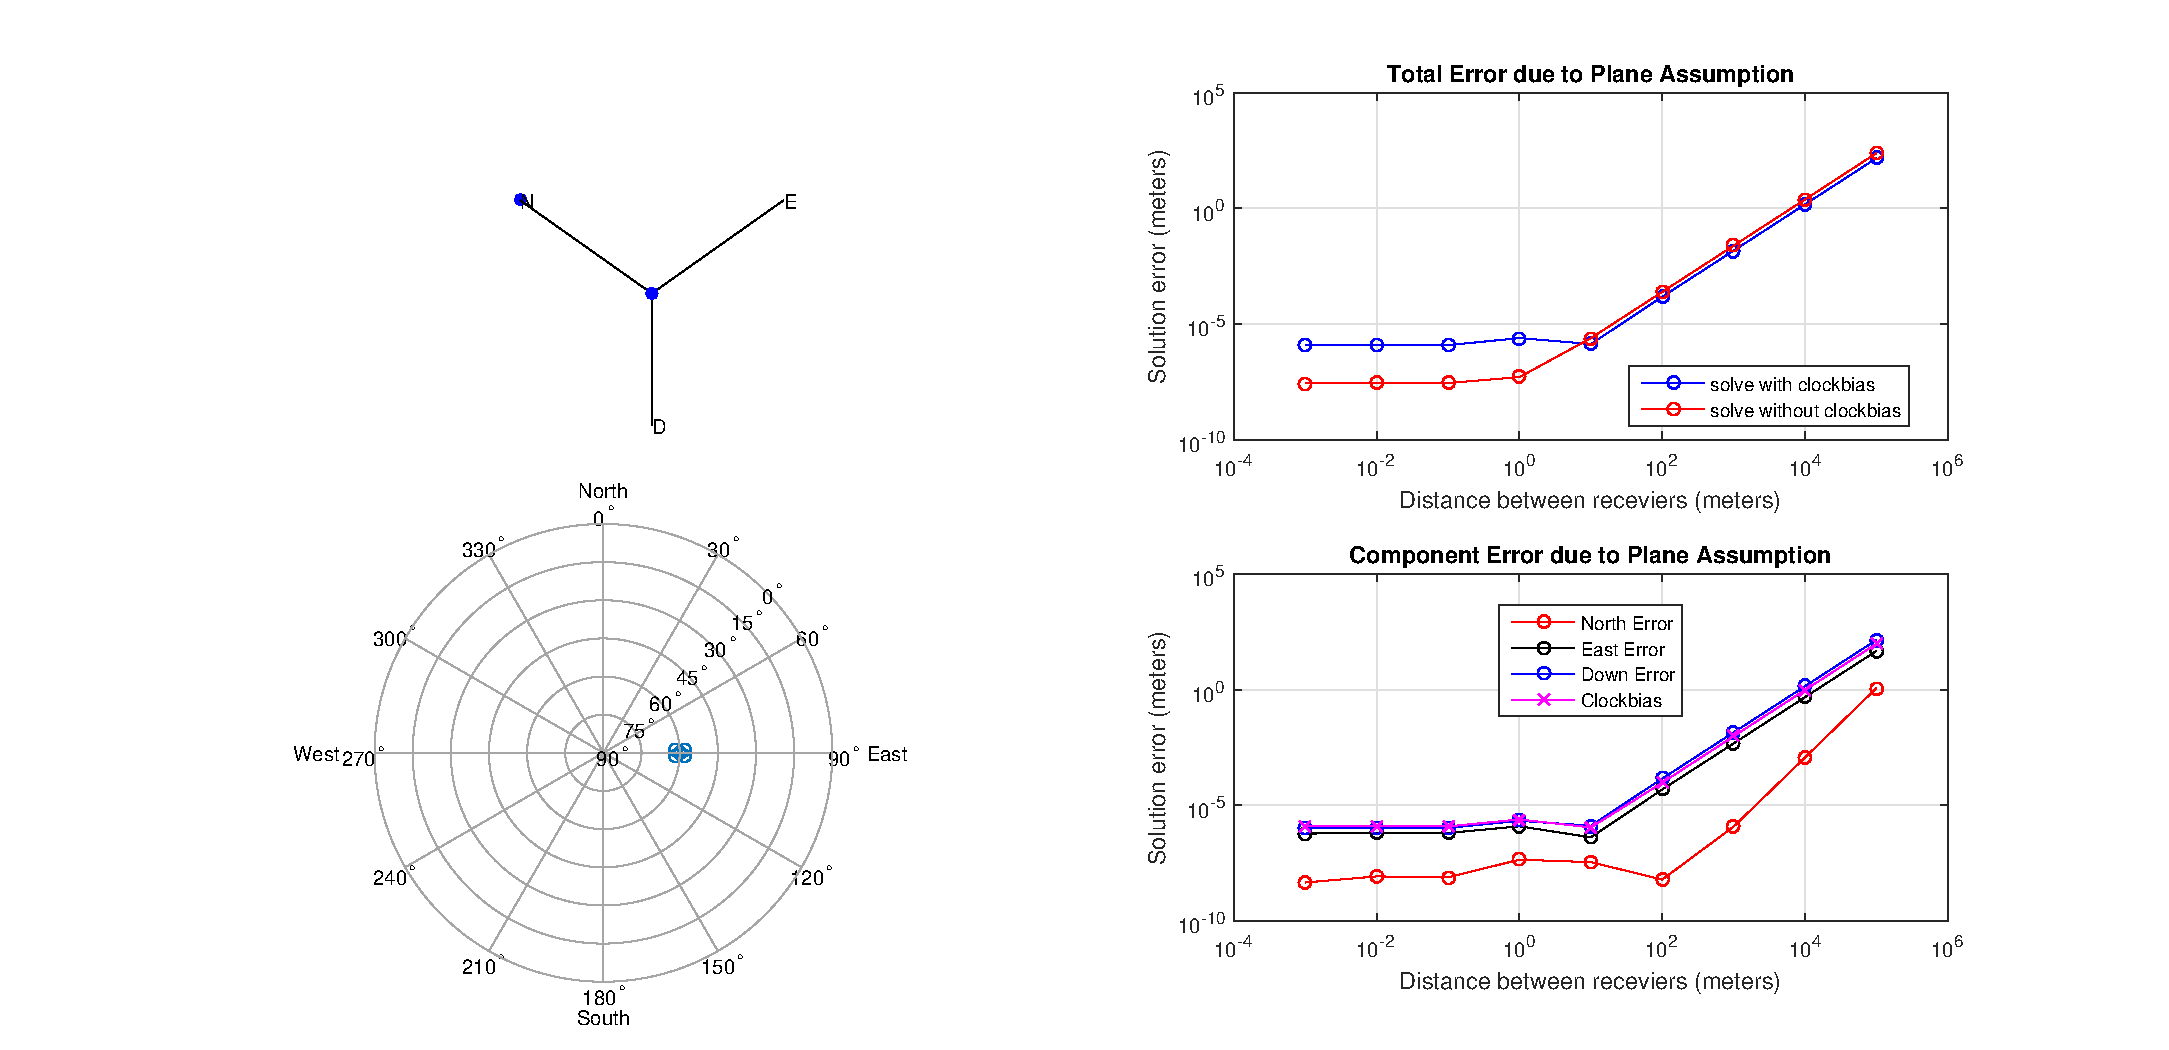
\includegraphics[trim = 3cm 0 0 0,clip,width=\linewidth]{ChapterExperiments/Figures/plane_ALLE_north_9060}
\end{figure}

The total error based on satellite configuration shown in Figure \ref{fig:plane_total_north1_pow4} for Northerly displaced receivers, Figure \ref{fig:plane_total_east_pow4} for East and Figure \ref{fig:plane_total_down_pow4} for Down. Note that the minimum for the Down configuration was 2 m whereas the minimum for the horizontal was 0.5 m. The down vector will inherently will have more error as the sphere curves up away from the plane assumption, however it is still in the same magnitude. It is due to the nature of the system, that the satellites are above the Earth, that PNT has less accuracy in the vertical plane than the horizontal plane as stated by the SPS Performance Standard \cite{officalperformance}. The north and east configurations are the same but $90^\circ$ out of phase. A full breakdown of which component causes the error is shown in Figure \ref{fig:plane_fullbreakdown}. High elevation causes the most error for both configurations, due to the down component, see (e) and (f) of Figure \ref{fig:plane_fullbreakdown}. The large error along the axis of the horizontal displacement, that is north for north and east for east, was due to the same direction, see (a). The orthogonal direction contributed significantly less error.\\

Based on this information, a satellite configuration was created to minimise the error due to the plane assumption in order to explore other affects.


\begin{figure}
\centering
\caption{}
\label{fig:plane_ALLE_north_0075}
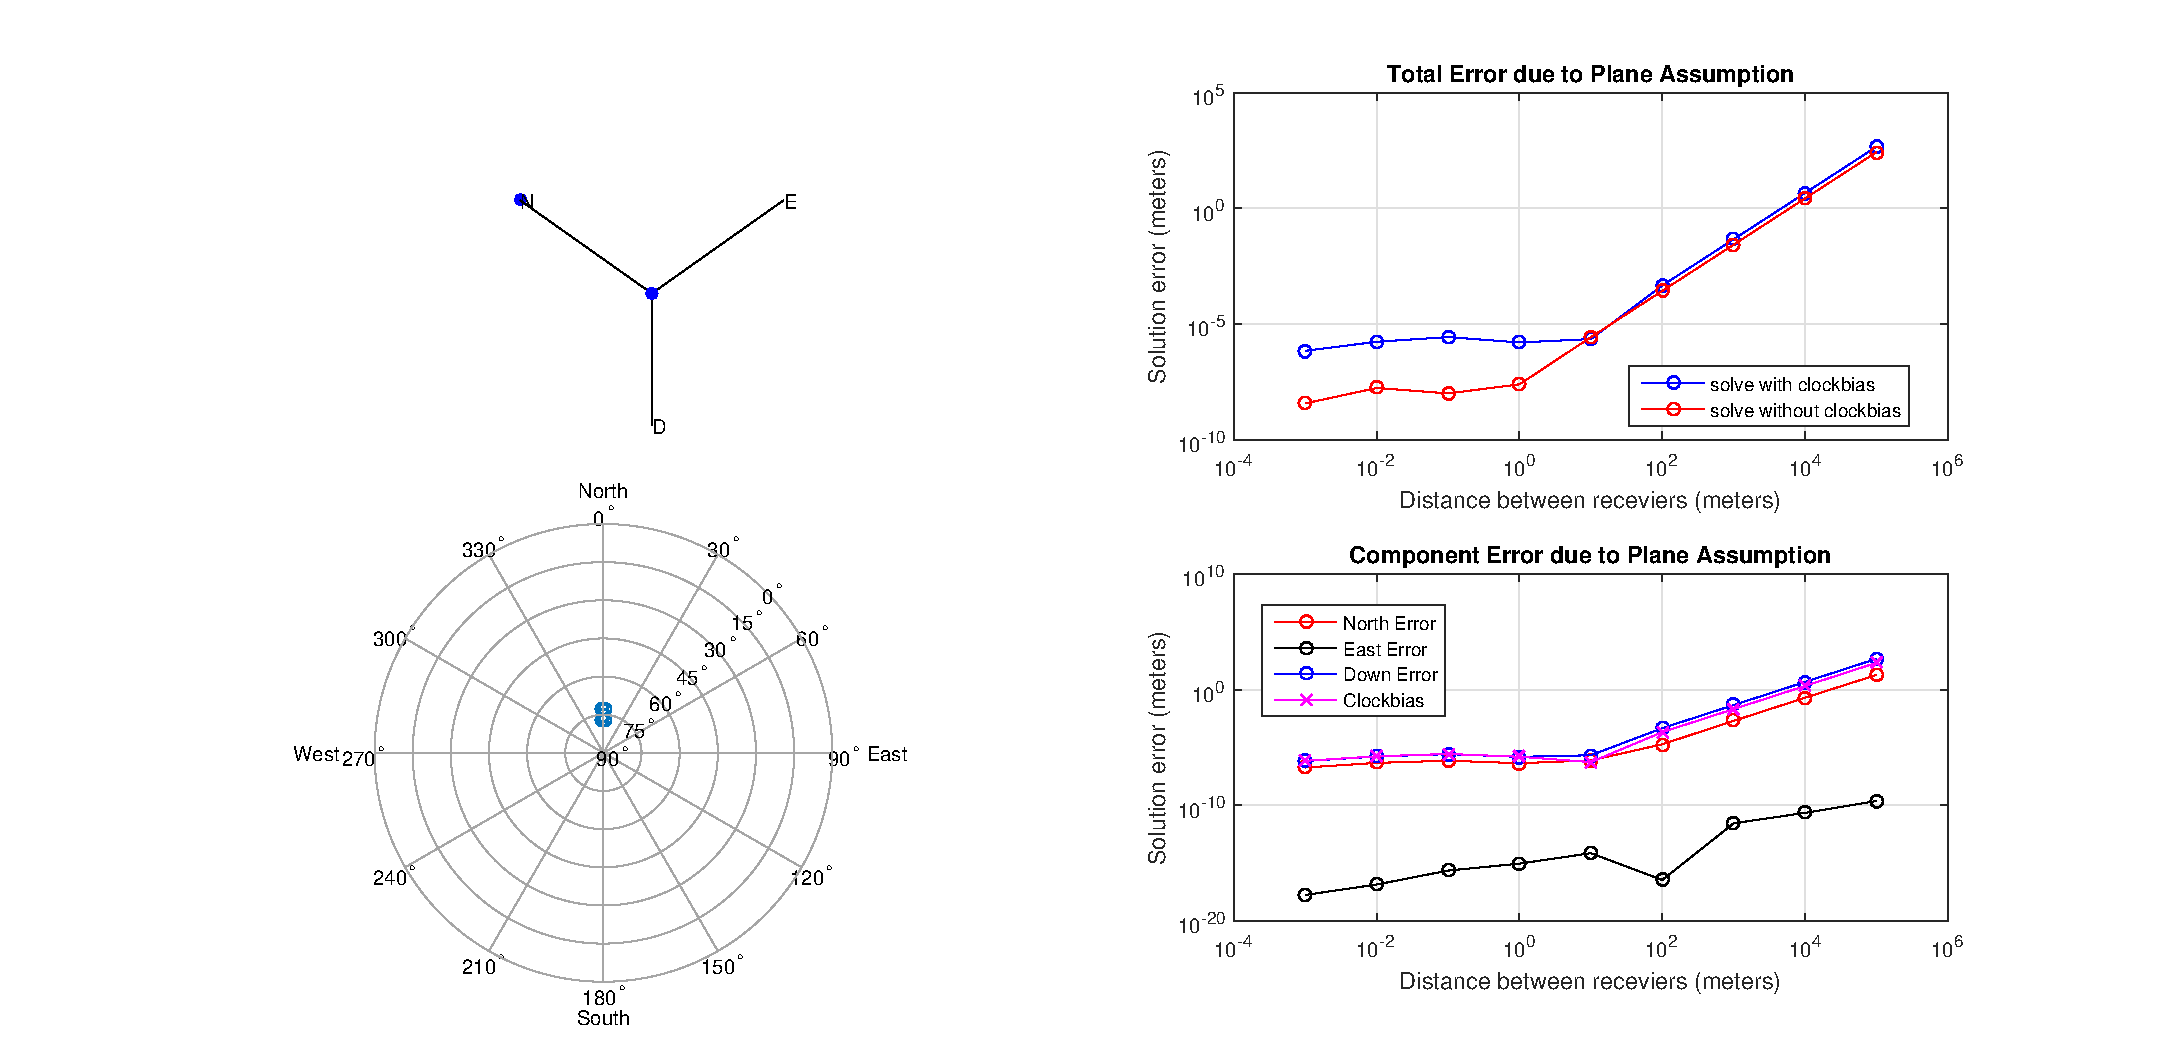
\includegraphics[trim = 3cm 0 0 0,clip,width=\linewidth]{ChapterExperiments/Figures/plane_ALLE_north_0075}
\end{figure}

%% using main_fn_planesats
\begin{figure}
\centering
\caption{NORTH: Total Error based on satellite configuration for two receivers 10 km apart along North vector}
\label{fig:plane_total_north1_pow4}
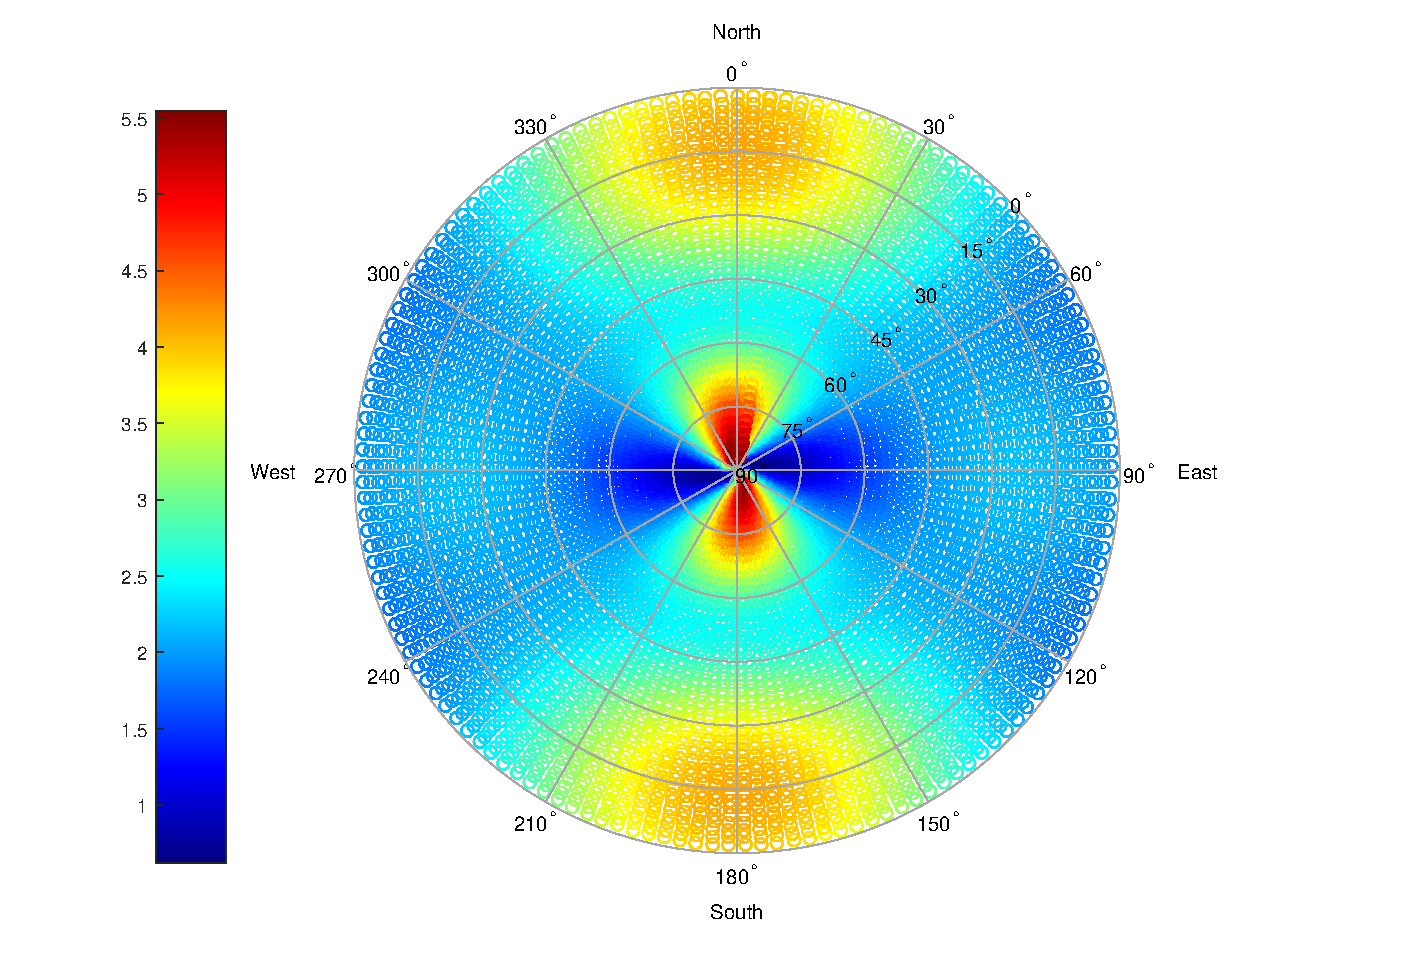
\includegraphics[width=0.7\linewidth]{ChapterExperiments/Figures/plane_total_north1_pow4}
\end{figure}

\begin{figure}
\centering
\caption{EAST: Total Error based on satellite configuration for two receivers 10 km apart along East vector}
\label{fig:plane_total_east_pow4}
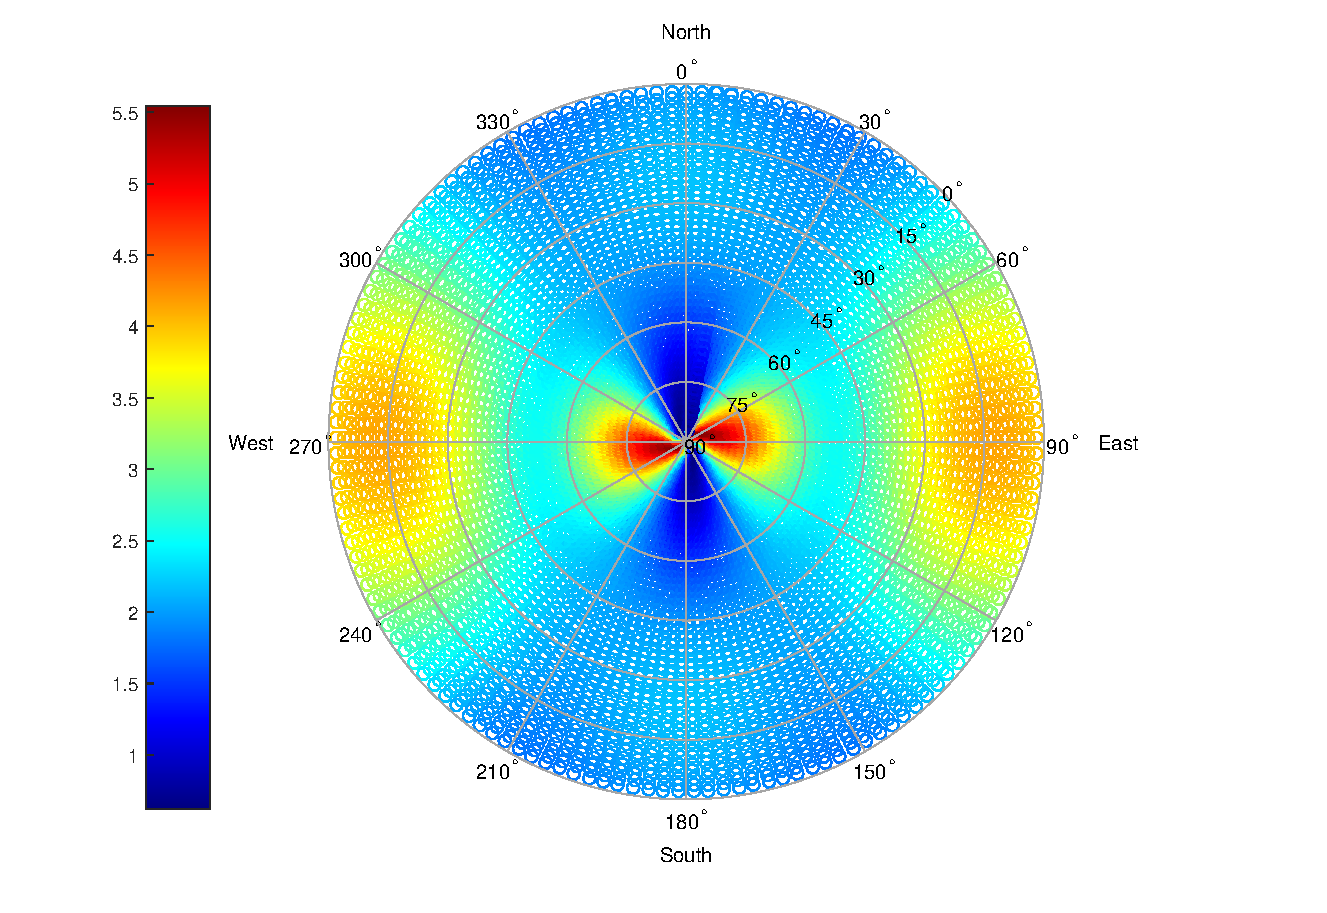
\includegraphics[width=0.7\linewidth]{ChapterExperiments/Figures/plane_total_east_pow4}
\end{figure}

\begin{figure}
\centering
\caption{DOWN: Total Error based on satellite configuration for two receivers 10 km apart along Down vector}
\label{fig:plane_total_down_pow4}
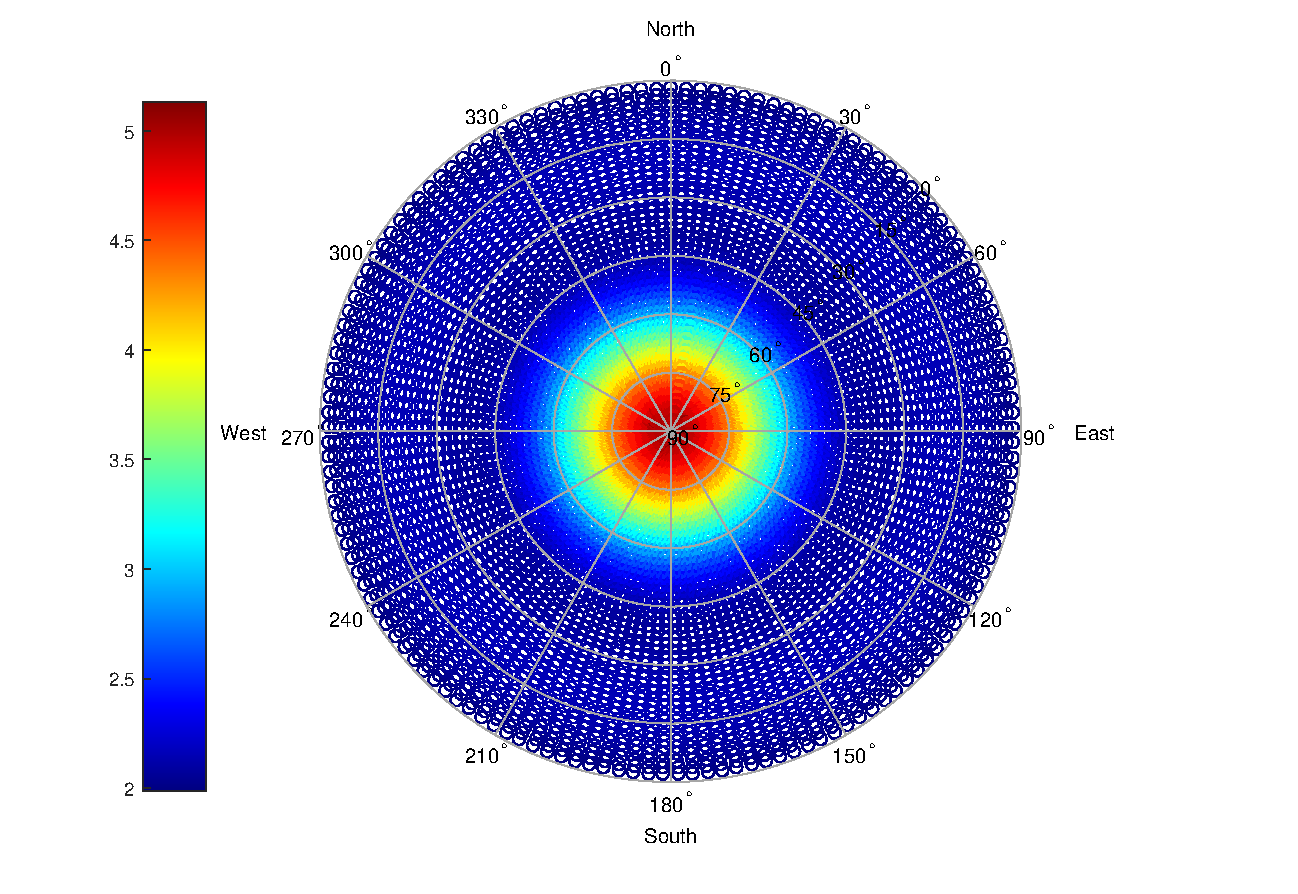
\includegraphics[width=0.7\linewidth]{ChapterExperiments/Figures/plane_total_down_pow4}
\end{figure}

\begin{figure}
\centering
\caption{Full breakdown of component error based on satellite configuration due to plane assumption (Note that not all the scales are the same but all are in meters)}
\label{fig:plane_fullbreakdown}
\begin{subfigure}[t]{0.49\textwidth}
\centering
\caption{Config:North, Error:North}
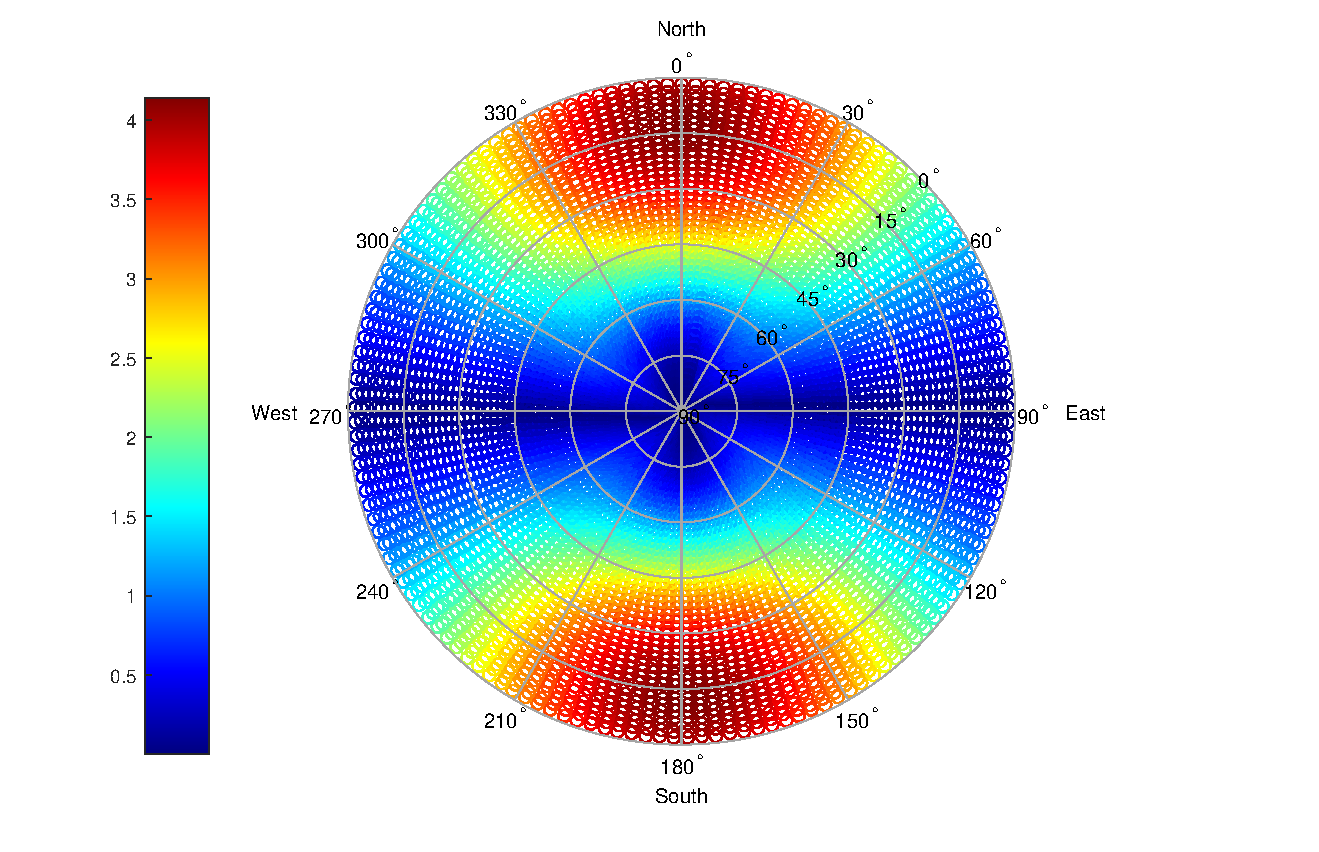
\includegraphics[width =\linewidth]{ChapterExperiments/Figures/plane_Enorth_north_pow4}
\end{subfigure}
\begin{subfigure}[t]{0.49\linewidth}
\centering
\caption{Config:Down, Error:North}
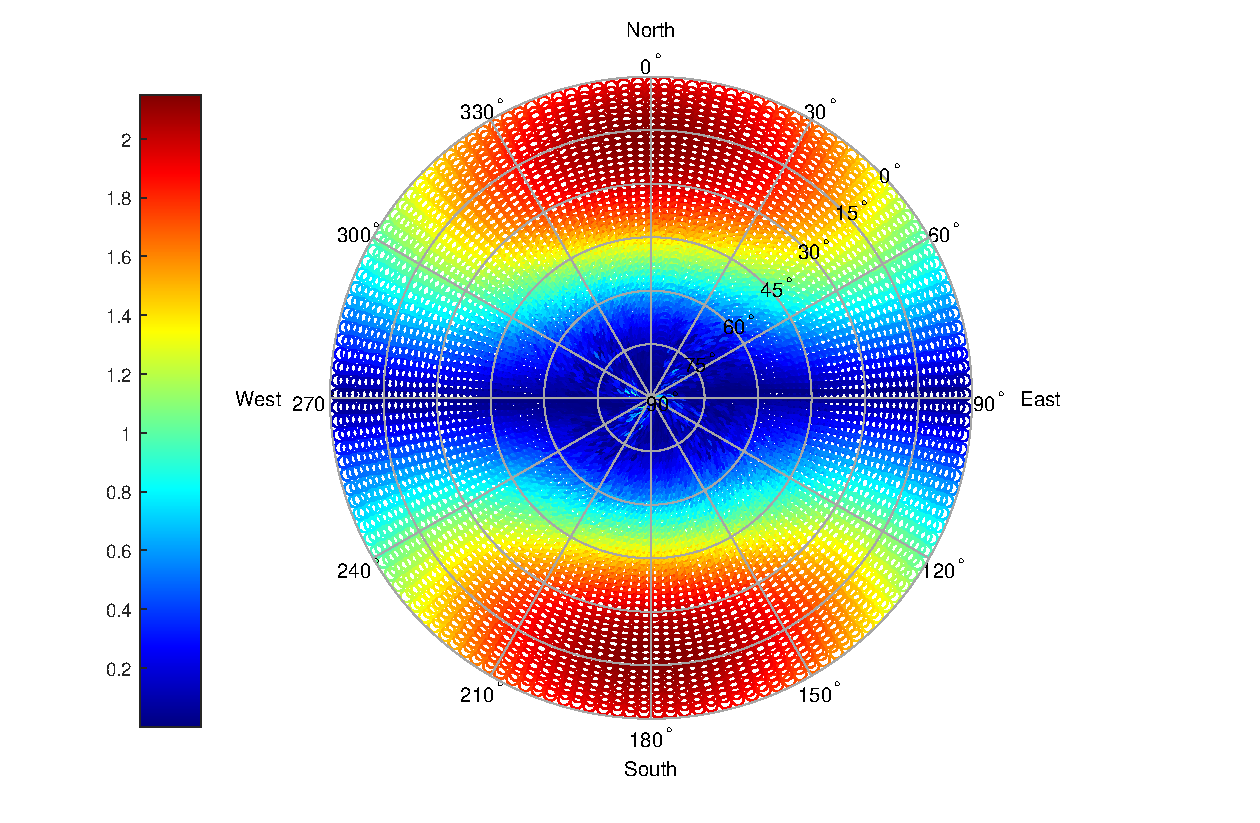
\includegraphics[width = \linewidth]{ChapterExperiments/Figures/plane_Enorth_down_pow4}
\end{subfigure}
\begin{subfigure}[t]{0.49\textwidth}
\centering
\caption{Config:North, Error:East}
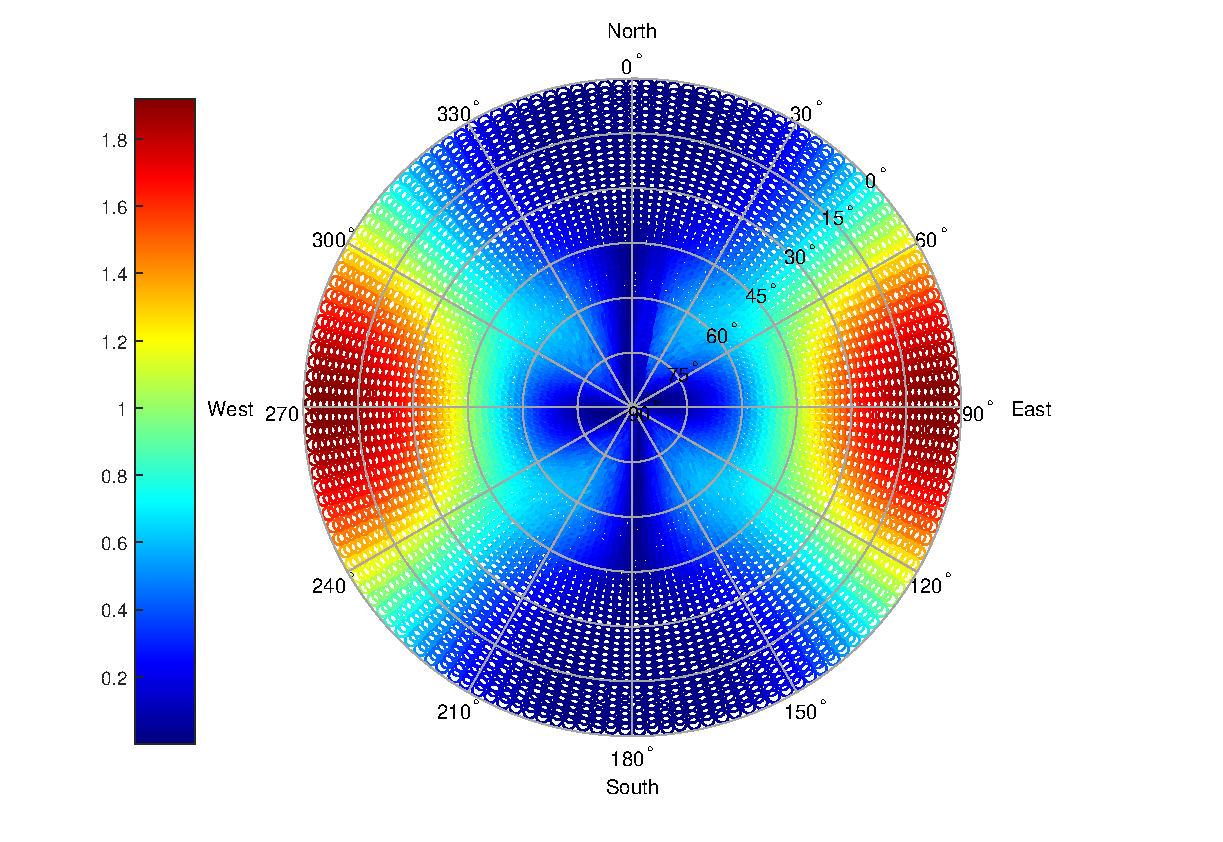
\includegraphics[width =\linewidth]{ChapterExperiments/Figures/plane_Eeast_north_pow4}
\end{subfigure}
\begin{subfigure}[t]{0.49\linewidth}
\centering
\caption{Config:Down, Error:East}
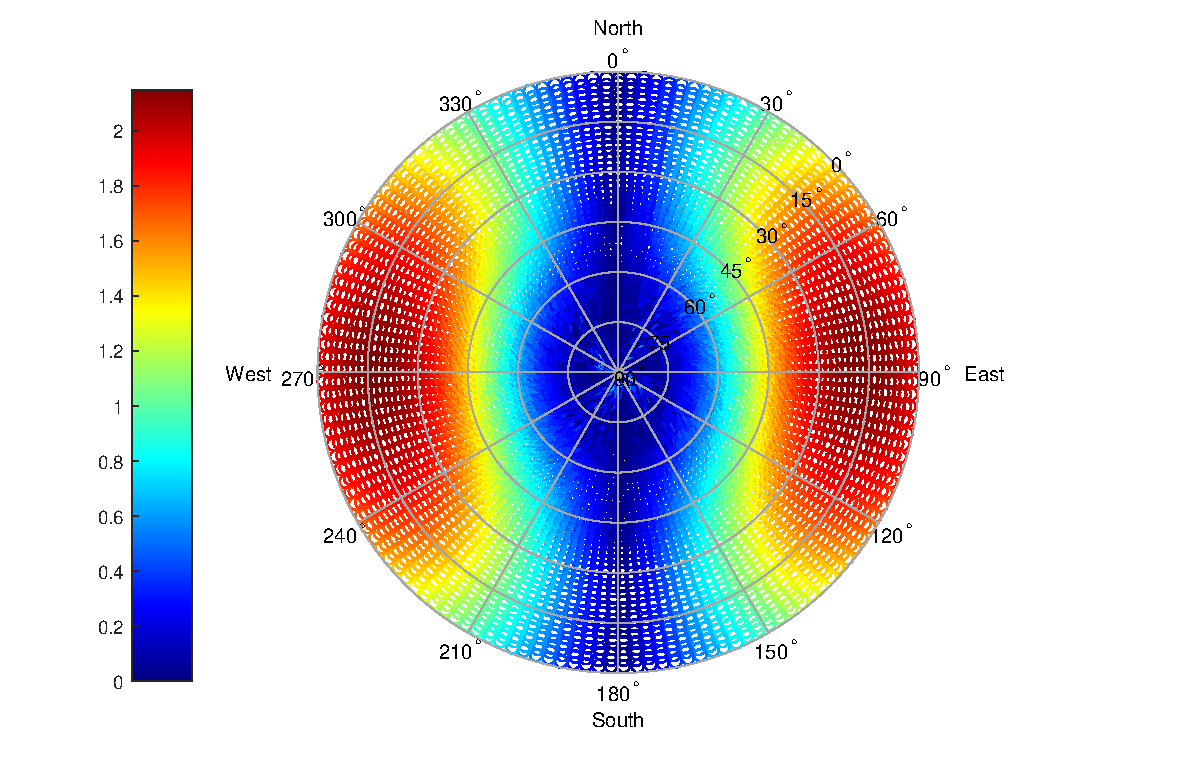
\includegraphics[width = \linewidth]{ChapterExperiments/Figures/plane_Eeast_down_pow4}
\end{subfigure}
\begin{subfigure}[t]{0.49\textwidth}
\centering
\caption{Config:North, Error:Down}
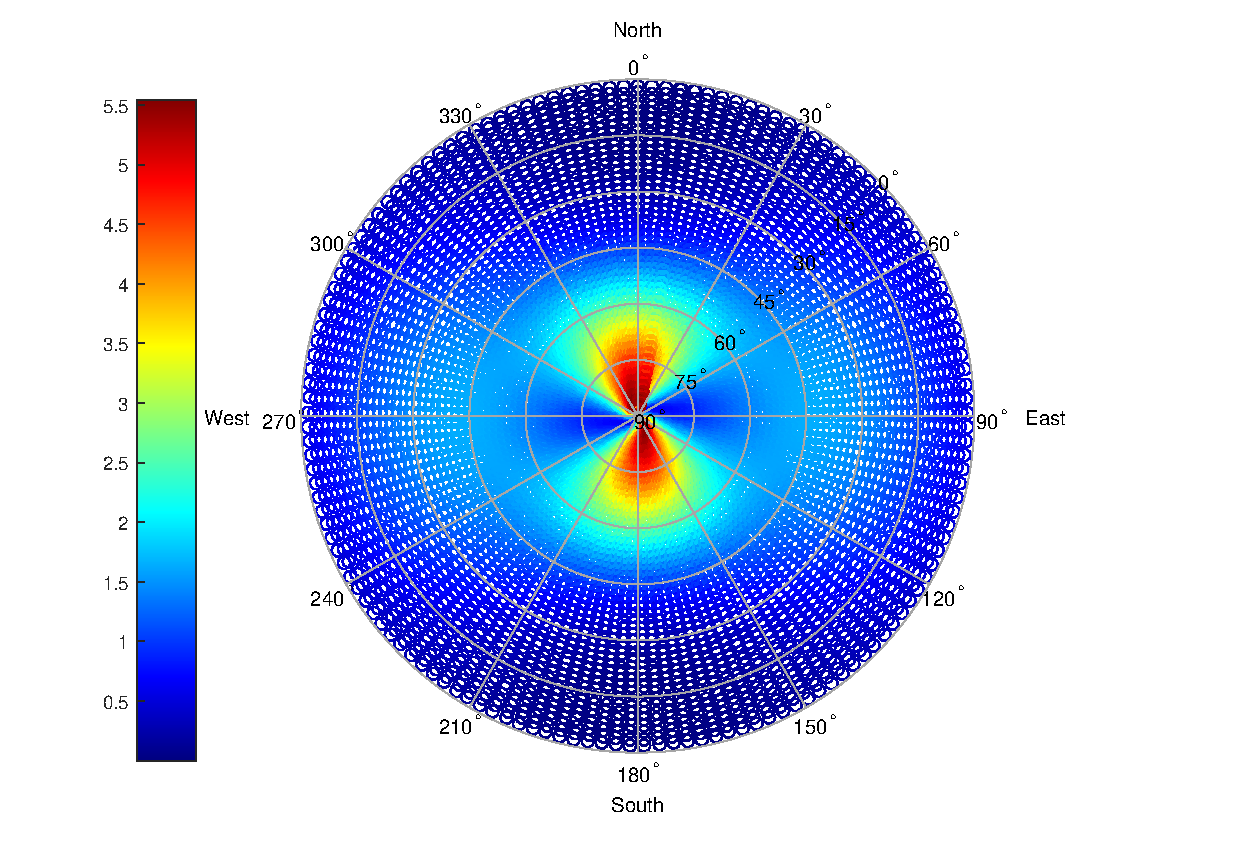
\includegraphics[width =\linewidth]{ChapterExperiments/Figures/plane_Edown_north_pow4}
\end{subfigure}
\begin{subfigure}[t]{0.49\linewidth}
\centering
\caption{Config:Down, Error:Down}
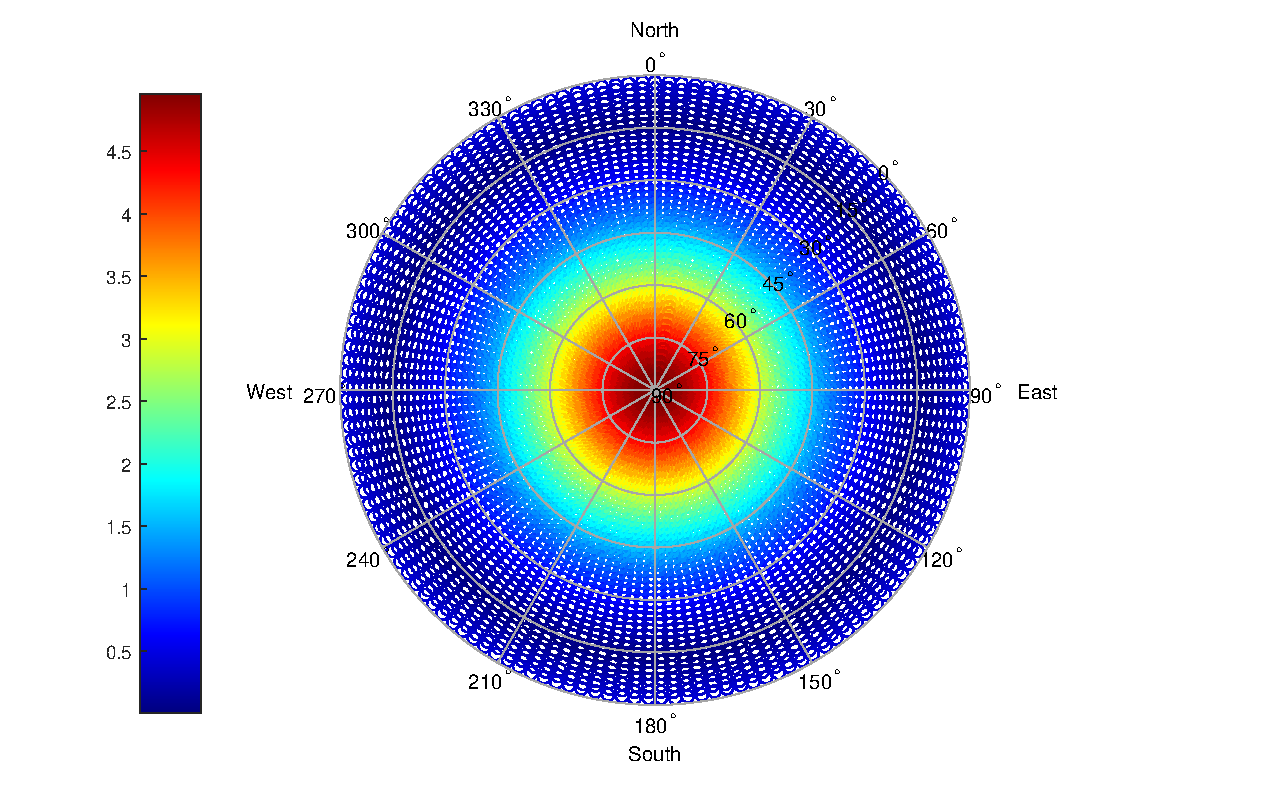
\includegraphics[width = \linewidth]{ChapterExperiments/Figures/plane_Edown_down_pow4}
\end{subfigure}
\end{figure}

%!TEX root = ../Thesis.tex

\section{Incorporating Error}
The error was systematically added in a randomly uniform fashion in three types of ways; satellite correlated error, receiver correlated error and random error. A statistically significant sample size of 100 iterations was conducted with the simulation using error created in Eq\eqref{Eq: errorstruc}. The planar algorithm was compared to NLLS using the same errors for each iteration. The mean and standard deviation were calculated. The satellite configuration for this section was Figure \ref{fig:satconfig_1m}.\\

The planar algorithm (PA) worked very well for satellite correlated errors, confirming the differential method of removing correlated errors, see Figure \ref{fig:Error_satellite}. The error for PA was consistent at $10^{-6}$ m, this lower limit was observed previously and is a product of the clock bias solution. Relative NLLS error increased linearly with the satellite correlated errors until it reached numerical instability.\\

PA also worked well at removing receiver correlated errors with an error of $10^{-6}$ m, however NLLS had better performance, see Figure \ref{fig:Receivers}. Large errors of $>10^{-3}$ seconds, which corresponds to a pseudorange error of $10^{-3}c = 298\; km$ might have the planar assumption effecting the solution.\\

Uncorrelated errors had the worst affect on the system, see Figure \ref{fig:Uncorellated}. But PA performed just as well as NLLS with error proportional to $c\times t$. This was expected as PA is based on removing errors by linear difference.

\begin{figure}
\centering
\caption{An Ideal Satellite Configuration for Northerly Displaced Receivers}
\label{fig:satconfig_1m}
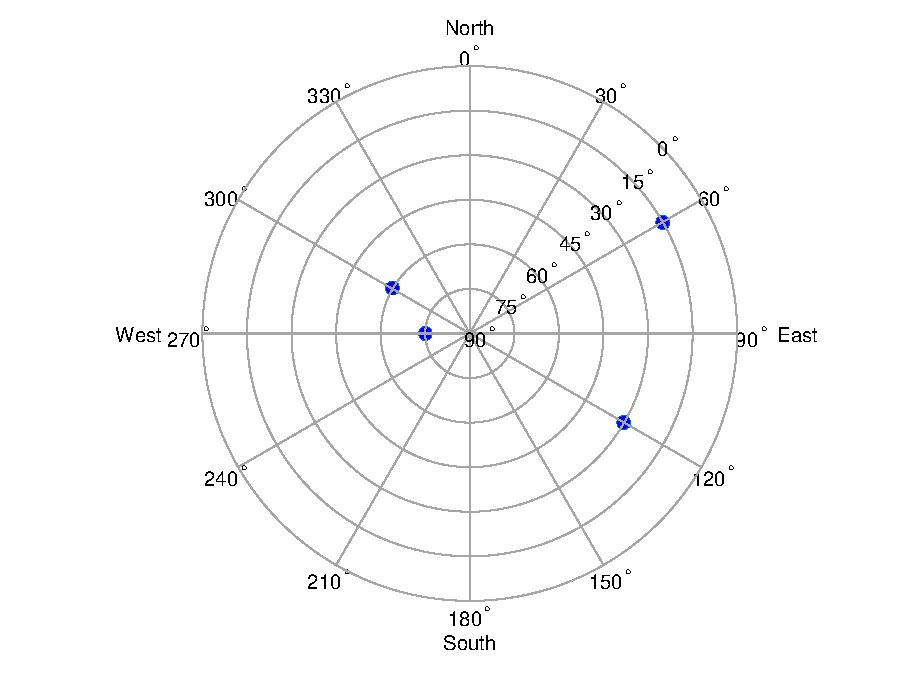
\includegraphics[width=0.7\linewidth]{ChapterExperiments/Figures/ControlledError/satconfig_1m}
\end{figure}


\begin{figure}
\centering
\caption{}
\label{fig:Error_satellite}
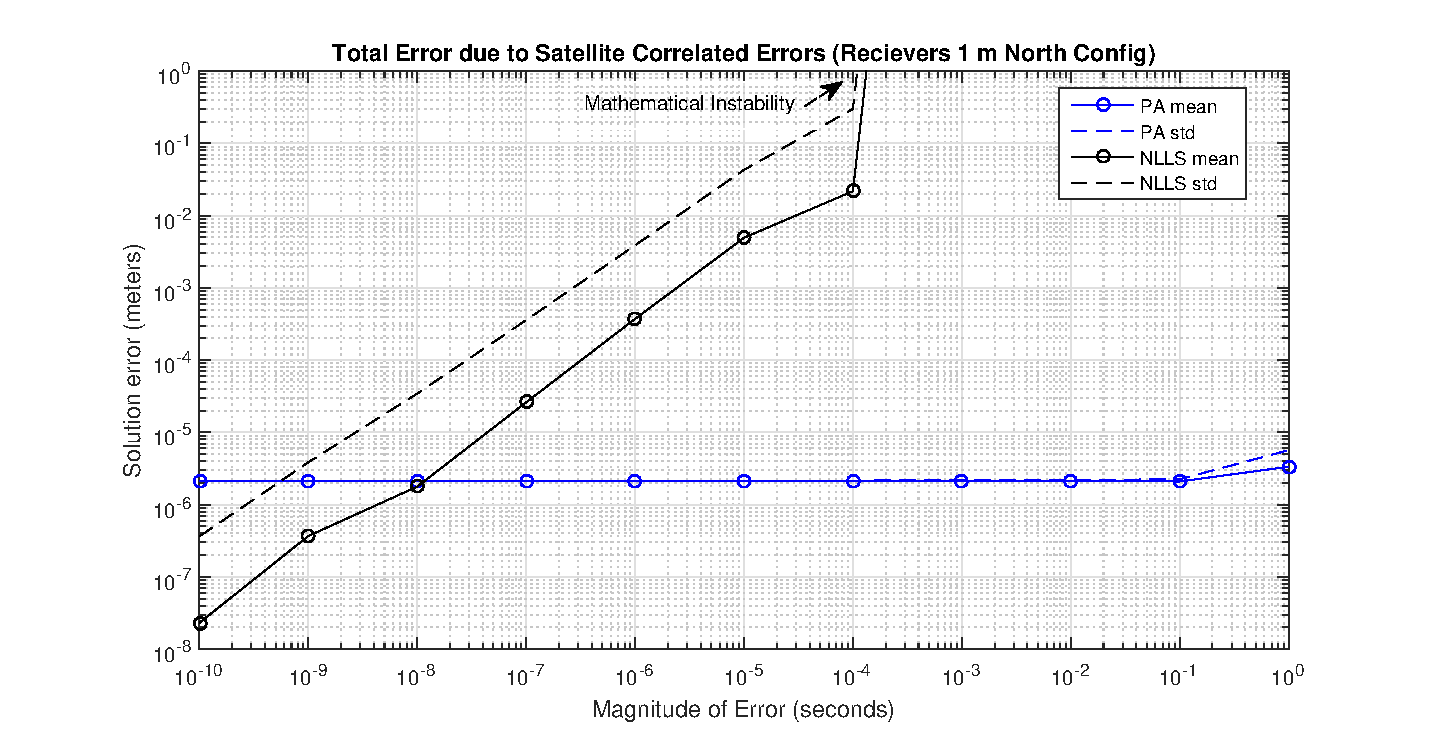
\includegraphics[width=1\linewidth]{ChapterExperiments/Figures/ControlledError/satellite}
\end{figure}

\begin{figure}
\centering
\caption{}
\label{fig:Receivers}
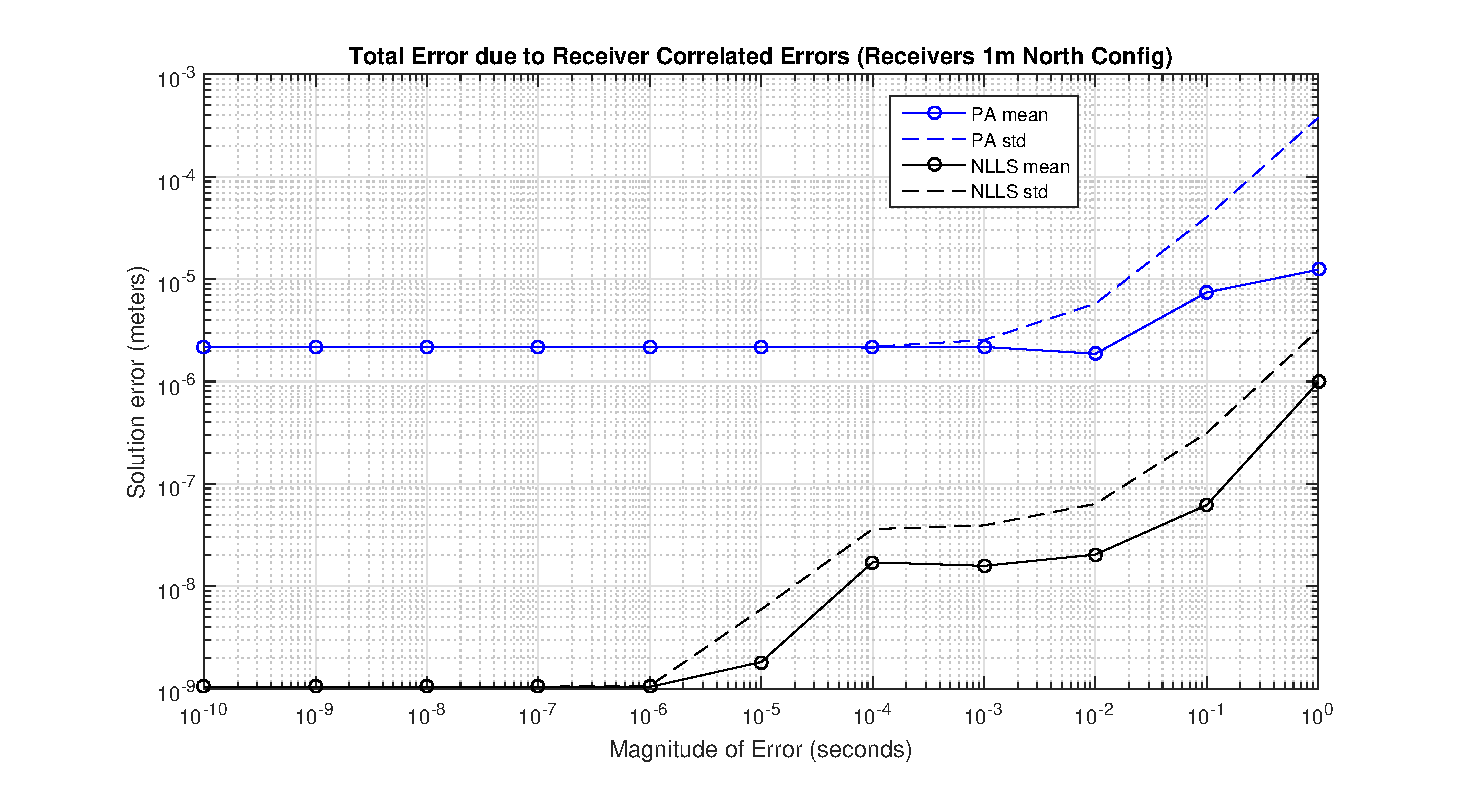
\includegraphics[width=1\linewidth]{ChapterExperiments/Figures/ControlledError/Receivers}
\end{figure}
\begin{figure}
\centering
\caption{}
\label{fig:Uncorellated}
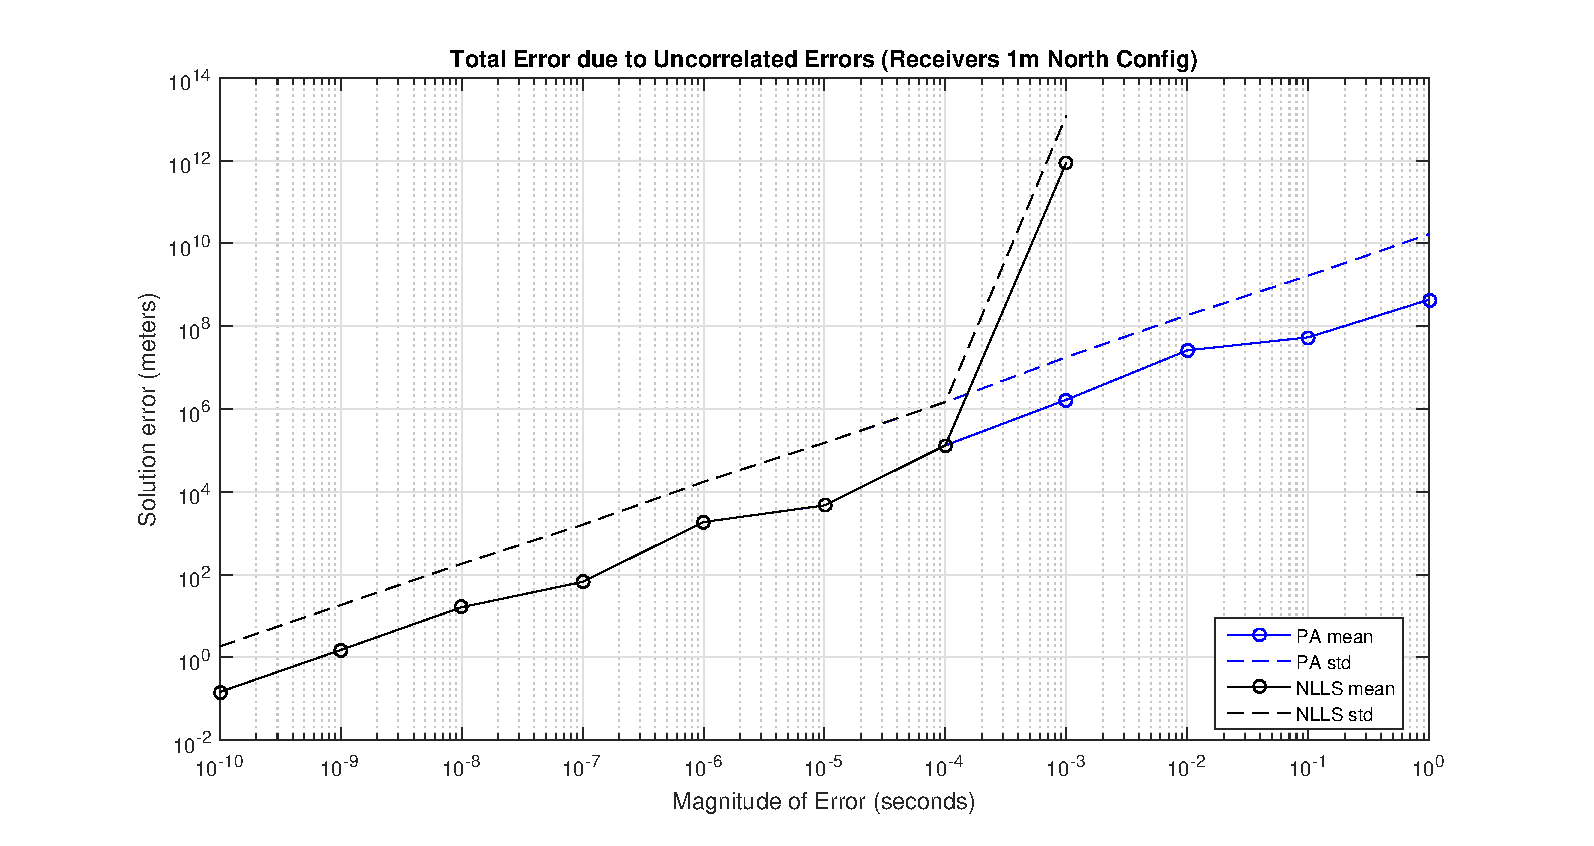
\includegraphics[width=1\linewidth]{ChapterExperiments/Figures/ControlledError/Uncorellated}
\end{figure}


 % may need to redo is it actually 10 m?
%\input{ChapterExperiments/Receiver} ??
%!TEX root = ../Thesis.tex
%%%%%%%%%%%%%%%%%%%% Conclusions %%%%%%%%%%%%%%%%%%%



			% Chapter 4
%!TEX root = ../thesis.tex

\def\chapdir{./ChapterConclusion}
\chapter{Conclusion}\label{ch:conclusion}

				% Chapter 5

%%==================== List of References ===================================%%
% Note that the List of References goes after the chapters but before the
% appendices. A Bibliography can contain references that are general
% background reading and are not cited in the text. A References or List of
% References section must contain only references that are cited in the text.
% Change to "Bibliography" in commands.tex if you wish and if appropriate.
\cleardoublepage

\begin{singlespace}

    \phantomsection
    \addcontentsline{toc}{chapter}{List of References}  % or "Bibliography"

    % acfrplainnat is a slightly modified version of plainnat from the natbib package.
    % I (AH) removed URLs from the output, since this seems unnecessary or a poorly
    % used field, and adjusted 'misc' to make more sense for the way I used it.

    % Bibliography styles supported by this template are apa-like (default) and ieee
    \bibliographystyle{ieeetrans}
    %\ifthenelse{\equal{\tReferenceStyle}{ieee}}
        %{\bibliographystyle{BibTeX/acfrplainnat}}    % IEEE-like style (or use plainnat)
        %{\bibliographystyle{BibTeX/apalike}}         % APA-like style (or use apalikeAkkaNat)

    \begin{raggedright}     % because you often get ugly whitespace if justified...
        \bibliography{BibTeX/thesis_bib}
    \end{raggedright}

\end{singlespace}

%%==================== Appendices ===========================================%%
% Appendices are almost exactly the same as chapters; the only difference is
% that they come after the \appendix command below.
\appendix 		% Switches from 'Chapter #' to 'Appendix X' chapter titles
%!TEX root = ../Thesis.tex

% This is to set the directory this chapter resides in for images
\def\chapdir{./AppendixSomething}

% Title of this chapter
\chapter{An Example Appendix}\label{ap:something}

As an appendix, this should contain some content that's not really required for the argument in the main body of the thesis, but is clearly relevant and supports the work.

%%!TEX root = ../Thesis.tex

\section{Code Listings}\label{sec:code}

The \texttt{listings} package allows you to include code listings or other formatted text with some parsing to make them more readable than simply calling \texttt{\textbackslash{}input\{\}} on the code file.

\definecolor{listinggray}{gray}{0.97}
\lstset{language=matlab}
\lstset{basicstyle=\scriptsize}
%\lstset{backgroundcolor=listinggray,framerulecolor=blue}
%\lstset{backgroundcolor=listinggray,rulecolor=blue}
\lstset{backgroundcolor=\color{listinggray},rulecolor=\color{blue}}
\lstset{linewidth=\textwidth}
%\lstset{labelstep=10}
%\lstset{commentstyle=\textit, stringstyle=\upshape,stringspaces=false}
%\lstset{commentstyle=\textit, stringstyle=\upshape,showspaces=false}
\lstset{commentstyle=\textit}
\lstset{frame=trbl,frameround=tttt}
\lstinputlisting[caption=\textsc{Matlab} script for interactive radians to degrees converter,label=lst:jacobians]{\chapdir/code.m}

A number of languages are supported with basic syntax highlighting and formatting.



%%!TEX root = ../Thesis.tex

\section{Multi-Page Tables}\label{sec:multipagetables}

The \texttt{supertabular} package allows tables to span multiple pages using
the \texttt{supertabular} environment (in place of \texttt{tabular}). This has
already been used in the \hyperref[fr:notation]{Nomenclature Section} in the
front matter, allowing the notation to span multiple pages if necessary.
\Autoref{tab:supertabex} shows an example of a table spanning two pages. Note
that such tables are no longer floating elements (i.e.~there's no
\texttt{table} environment anymore), and the header/footer for the whole
table, and ones repeated on each new page, can be defined through
\texttt{supertabular} macros rather than as part of the table to copy headers
across each page.

% Note that it's not in a table environment, since this is NOT a floating environment
\begin{center}
    % Use the supertabular commands rather than the usual caption/etc commands, since they are
    % inserted by supertabular
    \tablecaption[Page-Spanning `Super Table']{This table is especially long, so it's been turned
        into a \texttt{supertabular} environment allowing it to span multiple pages.
        \label{tab:supertabex}}
    % headers and footers can be defined to repeat on each page
    % firsthead and lasttail will be used INSTEAD OF the basic head/tails where appropriate
    \tablefirsthead{%
        \toprule
        \textbf{first} & \textbf{second} & \textbf{RHS}\\
        \midrule[1pt]
    }
    \tablehead{%
        \multicolumn{3}{l}{\small\sl continued from previous page}\\
        \toprule
        \textbf{first} & \textbf{second} & \textbf{RHS}\\
        \midrule
    }
    \tablelasttail{%
        \bottomrule
    }
    \tabletail{%
        \bottomrule
        \multicolumn{3}{l}{\small\sl continued on next page}\\
    }
    % Note that this is JUST the data in the table, since supertabular constructs multiple tables
    % using the firsthead/head/lasttail/tail definitions
    \begin{supertabular}{c @{$\times$} c @{$=$} c}
        1 & 1 & 1 \\
        1 & 2 & 2 \\
        1 & 3 & 3 \\
        1 & 4 & 4 \\
        1 & 5 & 5 \\
        1 & 6 & 6 \\
        1 & 7 & 7 \\
        1 & 8 & 8 \\
        \midrule
        2 & 1 & 2 \\
        2 & 2 & 4 \\
        2 & 3 & 6 \\
        2 & 4 & 8 \\
        2 & 5 & 10\\
        2 & 6 & 12\\
        2 & 7 & 14\\
        2 & 8 & 16\\
        \midrule
        3 & 1 & 3\\
        3 & 2 & 6\\
        3 & 3 & 9\\
        3 & 4 & 12\\
        3 & 5 & 15\\
        3 & 6 & 18\\
        3 & 7 & 21\\
        3 & 8 & 24\\
    \end{supertabular}
\end{center}

\section{Landscape Tables}\label{sec:landscapetables}

If your table is especially wide, it may be better to switch it to the landscape orientation. One way of doing this is with the \texttt{rotating} package, which implements (among other things) two new environments: \texttt{sidewaystable} and \texttt{sidewaysfigure}\footnote{I find \texttt{sidewaysfigure} less useful, as it tends to be easy enough to rotate the figure before inclusion, but if the caption/figure are complex it may be useful to have them oriented in the same way}. The way this package achieves this is most useful for \emph{printed results}, as it only rotates the environment on the page (but does not convert the page into landscape orientation)---for electronic viewing of a PDF, it may be useful to rotate the whole page since it's not often easy for the reader to rotate their screen (assuming the sideways content takes up the whole page). One advantage of this package's implementation of sideways environments is that it supports \texttt{twoside} page layout, and will rotate the sideways environment such that the bottom is towards the outside of the double-page layout in such cases.

An example of a \texttt{sidewaystable} is shown in \autoref{tab:sidewaystable}---if you're reading this as a PDF on your computer, you'll probably find it difficult to read as it's sideways on your
screen.

\begin{sidewaystable}
  \begin{center}
    \caption[Table in Landscape Orientation]{This table is so wide that I decided it should be in
        the landscape orientation to allow it to fit nicely on one page. You may of course find it
        easier (for the reader) to reconsider the content and layout of the table, or convert it to
        a graphical representation, as large walls of data tend to be hard to really interpret well.
        Almost certainly, you'd only have such large tables in an appendix.}
    \label{tab:sidewaystable}
    {\tiny
        % tiny font size because even sideways it wouldn't all fit at the normal font size
        % Note that the {\tiny ...} wraps the whole tabular environment.
    % This table is the output of a matlab script, which I found much easier than handwriting it all.
    \hspace{-14mm}  % HACK to move the table down on the page.
    \begin{tabular}{l c@{\hspace{4pt}}c @{\hspace{4pt}}c @{\hspace{4pt}}c @{\hspace{4pt}}c @{\hspace{4pt}}c @{\hspace{4pt}}c @{\hspace{4pt}}c @{\hspace{4pt}}c @{\hspace{4pt}}c @{\hspace{4pt}}c @{\hspace{4pt}}c @{\hspace{4pt}}c @{\hspace{4pt}}c @{\hspace{4pt}}c @{\hspace{4pt}}c @{\hspace{4pt}}c @{\hspace{4pt}}c @{\hspace{4pt}}c@{}}
      \toprule
      Item & Total &  1 &  2 &  3 &  4 &  5 &  6 &  7 &  8 &  9 & 10 & 11 & 12 & 13 & 14 & 15 & 16 & 17 & 18 \\
      \midrule
      SA Mission Distance (m) & 1101.4 & 49.4 & 81.5 & 34.2 & 78.8 & 98.8 & 70.8 & 16.0 & 61.4 & 14.9 & 52.1 & 24.3 & 83.3 & 170.3 & 143.5 & 20.7 & 30.1 & 21.4 & 99.2 \\
      SA Traversed Distance  (m) & 3244.1 & 53.9 & 86.8 & 90.7 & 92.1 & 120.8 & 74.3 & 46.4 & 63.8 & 15.6 & 55.3 & 27.4 & 127.2 & 222.4 & 987.1 & 273.0 & 167.0 & 235.4 & 505.0 \\
      MA Mission Distance (m) & 1083.9 & 59.1 & 81.5 & 34.2 & 78.8 & 98.8 & 70.8 & 16.0 & 61.4 & 14.9 & 52.1 & 24.3 & 83.3 & 170.3 & 143.5 & 20.7 & 30.1 & 21.4 & 81.8 \\
      MA Traversed Distance  (m) & 2343.1 & 61.8 & 84.6 & 70.7 & 84.6 & 116.6 & 72.5 & 46.3 & 62.6 & 15.5 & 53.5 & 25.8 & 129.4 & 213.4 & 147.1 & 268.2 & 174.5 & 233.8 & 482.3 \\
      \cmidrule(lr){2-20}
      Ratio (SA/MA) & 1.38 & 0.872 & 1.03 & 1.28 & 1.09 & 1.04 & 1.03 & 1 & 1.02 & 1.01 & 1.03 & 1.06 & 0.983 & 1.04 & 6.71 & 1.02 & 0.957 & 1.01 & 1.05 \\
      \midrule
      SA Mission Est. Time (s) & 734.3 & 32.9 & 54.4 & 22.8 & 52.5 & 65.9 & 47.2 & 10.7 & 40.9 & 9.9 & 34.8 & 16.2 & 55.5 & 113.5 & 95.7 & 13.8 & 20.1 & 14.3 & 66.2 \\
      SA Traversal Time  (s) & 2436.0 & 43.5 & 61.6 & 70.1 & 68.0 & 89.6 & 55.3 & 35.2 & 45.3 & 12.7 & 39.8 & 21.8 & 93.1 & 161.8 & 731.0 & 204.7 & 146.1 & 174.3 & 382.1 \\
      MA Mission Est. Time (s) & 1083.9 & 59.1 & 81.5 & 34.2 & 78.8 & 98.8 & 70.8 & 16.0 & 61.4 & 14.9 & 52.1 & 24.3 & 83.3 & 170.3 & 143.5 & 20.7 & 30.1 & 21.4 & 81.8 \\
      MA Traversal Time  (s) & 2411.3 & 64.2 & 84.8 & 73.6 & 86.8 & 119.1 & 74.2 & 47.2 & 63.5 & 16.1 & 54.3 & 28.1 & 132.8 & 215.2 & 148.2 & 271.3 & 203.4 & 239.9 & 488.7 \\
      \cmidrule(lr){2-20}
      Ratio (SA/MA) & 1.01 & 0.677 & 0.726 & 0.953 & 0.784 & 0.753 & 0.746 & 0.744 & 0.714 & 0.786 & 0.734 & 0.776 & 0.701 & 0.752 & 4.93 & 0.755 & 0.718 & 0.727 & 0.782 \\
      \midrule
      SA Cost (Exp.~Map)  & 1019924.1 & 1540.6 & 49041.0 & 5094.7 & 86202.5 & 98847.3 & 0.0 & 7974.8 & 1773.9 & 459.0 & 7825.8 & 1120.0 & 4131.3 & 14618.2 & 447306.7 & 19380.5 & 109612.1 & 33188.1 & 131807.7 \\
      MA Cost (Exp.~Map)  & 916661.5 & 6032.4 & 81939.1 & 7722.2 & 73856.9 & 198949.4 & 11654.8 & 6191.5 & 1398.9 & 564.8 & 13336.9 & 1123.8 & 6129.8 & 68857.2 & 39422.7 & 3213.2 & 172319.0 & 93562.5 & 130386.5 \\
      \cmidrule(lr){2-20}
      Ratio (SA/MA) & 1.11 & 0.255 & 0.599 & 0.66 & 1.17 & 0.497 & 0 & 1.29 & 1.27 & 0.813 & 0.587 & 0.997 & 0.674 & 0.212 & 11.3 & 6.03 & 0.636 & 0.355 & 1.01 \\
      \midrule
      SA Cost (Ground Truth)  & 26891.4 & 0.0 & 0.0 & 0.0 & 0.0 & 0.0 & 0.0 & 0.0 & 0.0 & 0.0 & 0.0 & 0.0 & 0.0 & 0.0 & 0.0 & 0.0 & 26891.4 & 0.0 & 0.0 \\
      MA Cost (Ground Truth)  & 28400.0 & 0.0 & 0.0 & 0.0 & 0.0 & 0.0 & 0.0 & 0.0 & 0.0 & 0.0 & 0.0 & 0.0 & 0.0 & 0.0 & 0.0 & 0.0 & 28400.0 & 0.0 & 0.0 \\
      \cmidrule(lr){2-20}
      Ratio (SA/MA) & 0.947 & -- & -- & -- & -- & -- & -- & -- & -- & -- & -- & -- & -- & -- & -- & -- & 0.947 & -- & -- \\
      \bottomrule
    \end{tabular}
    \begin{tabular}{l c c c}
    \noalign{\vspace{2ex}}
      \toprule
      Map Configuration & SA Coverage ($\textrm{m}^2$) & MA Coverage ($\textrm{m}^2$) & Ratio (MA/SA) \\
      \midrule
      Expanded Cost Map &   28108 &   28229 &     1 \\
      \bottomrule
    \end{tabular}
    }
  \end{center}
\end{sidewaystable}



%%!TEX root = ../Thesis.tex

\section{Including the PDF of a Relevant Paper}\label{ap:relevantPaper}

Occasionally it may be useful to include whole pages from another document in your thesis, where, for some reason, it is inappropriate or highly inconvenient to convert this into content yourself. This could apply to pages from a technical manual (which would be especially difficult for the average reader to track down), or a highly relevant paper you've published in the field, but not exactly on the thesis topic.

Inclusion of a separate PDF at the page level (rather than just as a floating figure) can be achieved using the \texttt{pdfpages} package\footnote{Please note that there appears to be a namespace clash between the \texttt{pdfpages} and \texttt{graphicx} packages. Including \texttt{pdfpages} \emph{after} \texttt{graphicx} resolves the issue.}. As an example, (three pages of) ``$P \neq NP$'', by Vinay Deolalikar, in its original form are embedded on the following pages.
% Make sure that you cite the paper correctly, and have a very good reason for including it verbatim in this manner!

\includepdf
[
    pages=1-3,      % For all pages, simply use the dash on its own: '-'
    % The pagecommand option adds a header over the top of the included PDF,
    % making it look like part of the thesis document. Here, it has been
    % copied from Thesis/Thesis.tex (so if you change that, you'll need to
    % copy it appropriately)
    pagecommand={\pagestyle{fancyplain}
        \lhead[\fancyplain{}{\thepage}]{\fancyplain{}{\rightmark}}
        \rhead[\fancyplain{}{\leftmark}]{\fancyplain{}{\thepage}}
        \cfoot{}},
    offset=0cm -0.5cm% Move the PDF downwards by 0.5cm.
    % There are many other options to shrink, rotate, etc.
]
{\chapdir/PneqNP}





\end{document}
